%!TEX TS-program = lualatex
%!TEX encoding = UTF-8 Unicode

\documentclass[oneside,12pt, letterpaper]{memoir}
%\usepackage{mathptmx}
\usepackage{semothesis}
\usepackage{amsmath}

\usepackage{graphicx}
	\graphicspath{{figs/}}

\usepackage{fontspec} 
\setmainfont[Ligatures={Common, TeX}, BoldFont={* Bold}, ItalicFont={* Italic}, BoldItalicFont={* BoldItalic}, Numbers={Proportional}]{Linux Libertine O}
\setsansfont[Scale=MatchLowercase,Ligatures=TeX]{Linux Biolinum O}
\setmonofont[Scale=MatchLowercase]{Inconsolatazi4}

\usepackage[protrusion=true, expansion=true]{microtype}
%
\usepackage{pdflscape}
\usepackage{pdfpages}
\usepackage{siunitx}
\usepackage{booktabs}
\usepackage{longtable}
\usepackage{threeparttable}
%\usepackage{float}
\usepackage{array}

\usepackage{url}
\makeatletter
\g@addto@macro{\UrlBreaks}{\UrlOrds}
\makeatother

% See https://tex.stackexchange.com/a/2652/39194
% Make this part of semothesis.sty
\makeatletter
\g@addto@macro\@floatboxreset\centering
\makeatother


\newcolumntype{W}[1]{>{\hangindent=6pt\raggedright\let\newline\\\arraybackslash\hspace{0pt}}p{#1}}

\newcolumntype{L}[1]{>{\raggedright\let\newline\\\arraybackslash\hspace{0pt}}p{#1}}
\newcolumntype{C}[1]{>{\centering\let\newline\\\arraybackslash\hspace{0pt}}p{#1}}
\newcolumntype{R}[1]{>{\raggedleft\let\newline\\\arraybackslash\hspace{0pt}}p{#1}}


%%  if you can get away without the default \DoubleSpacing, then
\setsemospacing{\OnehalfSpacing}


%% if you use endnotes, then
% \makepagenote

%\usepackage{lipsum}

%% Use them like this, and if you don?t change them you will
 %% get unacceptable title and/or approval pages
\settitle{Habitat Influence on Nesting Success of \textit{Lophodytes cucullatus} and \textit{Aix sponsa} (Aves: Anatidae) That Use Artificial Nest Boxes.}

\setauthor{Frank Jacob Irovic}

\setIDnumber{S02004278}

\masters  % going for a Masters degree

\emphasisarea{Biology}
\complementaryarea{}


\setgraddate{2025}

%\setcommitteechair{Michael S.~Taylor, Ph.D.}
%\setcommitteetwo{John S.~Scheibe, Ph.D.}
%\setcommitteethree{Philip W.~Crawford, Ph.D.}
%\setcommitteefour{}  % Use if you have a fourth committee member.


% Set to \forthMembertrue if committee has 4th person.
\fourthMemberfalse
%\fourthMembertrue

%\setdepartmentchair{James E.~Champine, Ph.D.}

%\setgraduatedean{Tamela D.~Randolph, Ph.D.}


%\hyphenation{Cteno-pharyng-o-don Hyp-oph-thalm-ichthys}
\newcommand{\nmds}{\textsc{nmds}}
\newcommand{\mergsci}{\textit{Lophodytes cucullatus}}
\newcommand{\woodsci}{\textit{Aix sponsa}}
\newcommand{\merg}{Hooded Merganser}
\newcommand{\wood}{Wood Duck}

\newcommand{\ccby}[1]{%
	\ifx&#1&
	{\textsc{cc by}}%
	\else
	{\textsc{cc by #1}}
	\fi}


\newcommand{\ccbysa}[1]{%
	\ifx&#1&
	{\textsc{cc by-sa}}%
	\else
	{\textsc{cc by-sa #1}} 
	\fi}

\newcommand{\ccbyncsa}[1]{%
	\ifx&#1&
	{\textsc{cc by-nc-sa}}%
	\else
	{\textsc{cc by-nc-sa #1}}
	\fi}

\newcommand{\ccbync}[1]{%
	\ifx&#1&
	{\textsc{cc by-nc}}%
	\else
	{\textsc{cc by-nc #1}}
	\fi}

\newcommand{\ccbyncnd}[1]{%
	\ifx&#1&
	{\textsc{cc by-nc-nd}}%
	\else
	{\textsc{cc by-nc-nd #1}}
	\fi}

\newcommand{\cc}{%
	\textsc{cc0}%
}

\begin{document}

\maxtocdepth{subsection} % put 3 levels into the ToC

\frontmatter
\thetitlepage
\copyrightpage
%\oldapprovalpage

\IfFileExists{thesis-acceptance-sheet.pdf}
{
	\includepdf{thesis-acceptance-sheet}
}{
	\newgeometry{left=1in, right=1in, top=1in, bottom=0.9in}
	\setlrmarginsandblock{1in}{1in}{*}
	\newlength{\temptop}
	\newlength{\tempbottom}
	\setlength{\temptop}{\uppermargin}
	\setlength{\tempbottom}{\lowermargin}
	
	\setlength{\uppermargin}{1in}
	\setlength{\lowermargin}{0.9in}
	\checkandfixthelayout[nearest]
	
	\OnehalfSpacing
	
	\approvalpage
	
	\setsemospacing{\SemoSpacing}
	
	\restoregeometry
	\setlrmarginsandblock{1.5in}{1in}{*}
	\setlength{\uppermargin}{\temptop}
	\setlength{\lowermargin}{\tempbottom}
	\checkandfixthelayout[nearest]
}


%% if you have a dedication, then it will appear here.
\IfFileExists{dedication.tex}{%
\semodedication
 	%!TEX encoding = UTF-8 Unicode

The entirety of my academic work and especially this thesis is dedicated to my family and friends. To my friends for the countless good times and midnight conversations. To my brothers, Anthony who never fails to be the ultimate example of hard work and Joe who reminds me that taking time for what’s most important is just as valuable. To Sara for her unending love and encouragement through any and all stressful times. I have special gratitude for my parents who introduced me to and nurtured my love of the outdoors.  It is because of your love, support, patience, and guidance that I have been able to work and grow in my education and in life. I could never find a better group of people to surround myself with. And finally to God, for creating the wild things and places where I find my passion. 
}%Don't include if it doesn't exist.

\semoacknowledgements
	%!TEX encoding = UTF-8 Unicode

I am thankful to many people but first and foremost to my advisor, Dr.~Michael Taylor. I have been fortunate to have his excellent guidance and direction throughout both my undergraduate and graduate academic experiences. His passion for his work has served as an inspiration and his recommendation was very important in pushing me to continue to a masters. He has been a force of growth for me as a scientist, student, and person. Not to mention his willingness to go above what is expected of an advisor. Without his help I don’t know if I would have made it through the final sprint. 

I am also thankful for my committee members, Dr.~Kelly Fritz and Dr.~Lucas Kirschman. Their guidance and suggestions have been essential to the completion of my project. They have both also served as great instructors, helping me to grow in my knowledge of wetlands, statistics, and the research process.  

This project would likely not have come to form without Nicole Walker of the Missouri Department of Conservation and later the U.S.~Fish and Wildlife Service. Her guidance and education is what introduced me to working around nest boxes and further grew my interest in the ducks that use them. It is this that sparked my interest in researching this topic. 

I am also grateful to the Missouri Department of Conservation and especially the staff at Duck Creek Conservation Area. Their hard work has ensured the existence of excellent wildlife habitat available to projects like mine, the public, and most importantly the wildlife that rely on it.  

\OnehalfSpacing

\tableofcontents*
\listoffigures  % if you have any figures
\listoftables   % if you have any tables

\setsemospacing{\SemoSpacing}

\pagestyle{semo}
\semoabstract
	%!TEX encoding = UTF-8 Unicode

Hooded Merganser and Wood Duck are ducks that reproduce by building nests in tree cavities. Cavities can be supplemented with artificial nest boxes to improve management success. Nest boxes should be placed in different habitats that facilitate feeding and reproduction of each species.  Hooded Merganser dive below the water to pursue fish and thus should prefer deeper water. Wood Ducks feed on the surface or dabble and thus should prefer shallower water. To test this hypothesis, 10 nest boxes were randomly selected from each of 3 pools at Duck Creek Conservation Area near Puxico, Missouri. For each nest box, water depth and width, and tree coverage were measured. Each nest box was monitored weekly to determine nesting species and number of eggs hatched. Dump nesting was also assessed. 

Water depth and tree coverage were significantly different for Pool 1 compared to the other two pools. Nests occurred in 17 of 30 nest boxes. Sequential nests occurred in 6 of these boxes for 23 nest events total. Hooded Merganser presence and success were generally associated with the deeper pools. Wood Duck presence was associated with the shallower pools, but this did not appear to affect nesting success. This suggests that water depth may influence nest box selection by these two species. Thus, consideration of water depth adjacent to nest boxes may be an important consideration for waterfowl biologists and conservation managers.  

% \semodedication{ text } % if you want a dedication

\mainmatter

\chapter{INTRODUCTION}
	%!TEX encoding = UTF-8 Unicode

Many waterfowl (Aves: Anatidae) species, like other groups of birds, have experienced population declines across North America, largely driven by habitat loss (Norton and Thomas~1994, Rosenberg et~al.~2019).  Active management to conserve North American waterfowl began during the late 19th century and has included international treaties, evolving hunting regulations, and public-private habitat manipulation (Williams et~al.~1999, Brasher et~al.~2019). As a result, population size of nearly 57\% of waterfowl species have increased, but more than 43\% remain in decline since 1970 (Rosenberg et~al.~2019). Annual fluctuation of population size for all waterfowl species suggests that continual monitoring and adjustments to management practices are still required  (Wilkins and Cooch~1999, Nichols et~al.~2007). 

	Successful waterfowl management requires detailed understanding of their reproductive biology but key aspects of the reproductive process are not fully understood. Accurate data at specific management locations are required for improvement (Nichols et~al.~1995, Hagy et~al.~2014). One location that has been continually managed for waterfowl reproduction is Duck Creek Conservation Area \textsc{(dcca)} in southeast Missouri. The area provides important foraging habitat during migration by controlling flooding to encourage plant growth. It also provides hollow tree cavities as well as nest boxes that mimic them to provide important spring nesting habitat for Hooded Merganser \textit{(Lophodytes cuculattus)} and Wood Duck \textit{(Aix sponsa).} To increase the understanding of waterfowl breeding at \textsc{dcca}, a study was conducted to compare nesting success by both species to habitat variables surrounding nest locations.  




\section*{Species background}

Hooded Merganser is a small diving duck (Figure~\ref{fig:hooded_merganser_photo}) native to North America. They are the only extant member of \textit{Lophodytes} and are most closely related to the typical mergansers of the genus \textit{Mergus}, such as the Common Merganser \textit{(M.~merganser)} and Red-breasted Merganser \textit{(M.~serrator)} in North America (Livezey 1995). Hooded Merganser is a small duck with a slender, serrated bill, and a pronounced crest on the head of both sexes. Females have a drab grey-brown body with a cinnamon crest. Males have a white chest, brown sides, a black back, and a black head with a prominent white patch on the crest. This crest can be raised or lowered in both sexes to alter the shape of the head and display a white color patch in males (Johnsgard 1961). 

\afterpage{%
\begin{figure}[p!]
	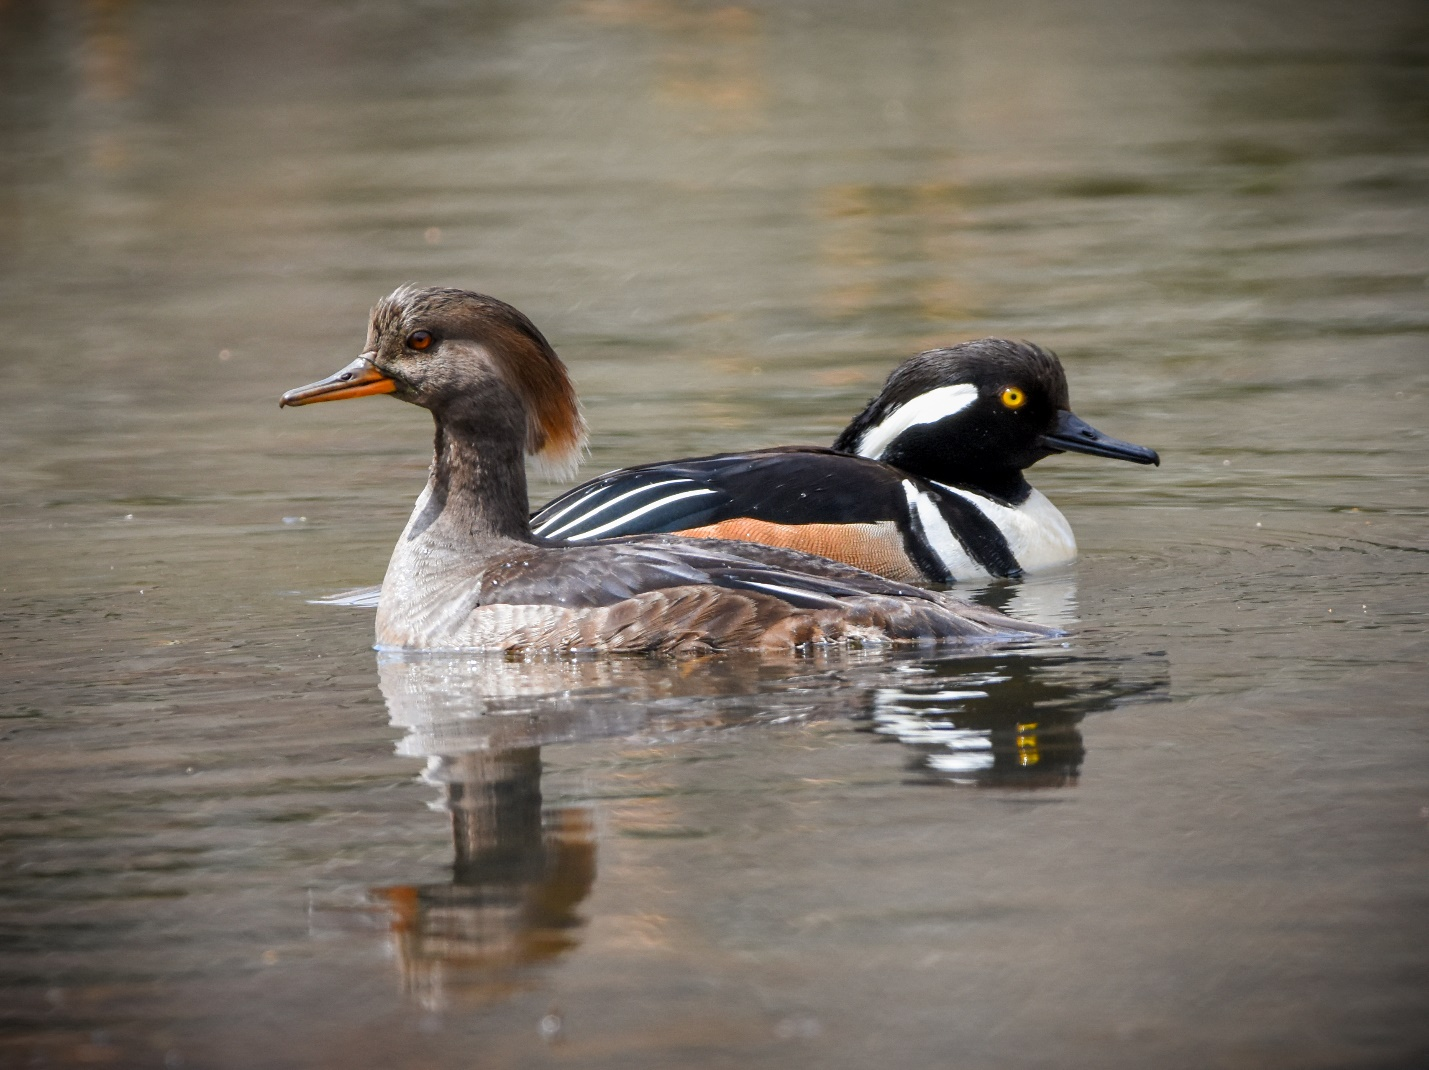
\includegraphics[width=\textwidth]{hooded_merganser_photo}
	\caption[Representative photo of Hooded Merganser]{Representative photo of Hooded Merganser hen (left) and drake (right). Photo by Jen Goellnitz, Flicker Creative Commons,  \ccbync{2.0}
	 \url{https://www.flickr.com/photos/goellnitz/33597600618/}.}
	\label{fig:hooded_merganser_photo}
\end{figure}
\clearpage}

 


Hooded Merganser dive below the water surface to sight feed for fishes, which dominate their diet, and invertebrates (Salyer and Lagler 1940, K. M. Dugger et~al.~1999). They favor water deep enough to support small fish or where they can swim below the surface, but their overall habitat includes ponds, rivers, large wetlands, and wooded swamps. The water bodies must have trees nearby because Hooded Merganser is a cavity nesters. Females lay eggs in hollow tree trunks above the ground or water. Courtship occurs before nesting and much earlier than other merganser species. The other, larger merganser species court during February, whereas Hooded Merganser begin courtship as early as November (Coupe and Cooke 1999). One male will pair with one female at least for the breeding season and egg laying will begin in March, earlier than many other cavity nesting waterfowl (Armbruster 1982, Rohwer and Anderson 1988, Soulliere and Rusch 1996, Rodway 2007). Hooded Merganser typically lays one clutch of 8–10 eggs per nesting season (Mallory et~al.~1998).  

Hooded Merganser has been negatively affected by habitat loss and alteration, largely due to clearcutting and draining fertile floodplain for industrial agriculture that results in the loss of permanent water and mature trees. As areas have been drained, Hooded Merganser has lost access to food sources. In areas not drained, timber harvesting and altered flood regimes have decreased the number of mature trees with suitable nesting cavities. Fewer cavities have reduced population growth compared to other waterfowl and seemingly increased the need for artificial nest boxes that mimic natural cavities to be included in management practices (Perry et~al.~2007).

One species competing with Hooded Merganser for nesting cavities is the Wood Duck.  Wood Duck is a small dabbling duck endemic to North America. Wood Duck is the only species of \textit{Aix} in North America. The only other species in the genus, the Mandarin Duck \textit{(Aix gtalericulata)}, is endemic to eastern Asia but is the sister species to Wood Duck (Liu et~al.~2014). Wood Duck have a short wide bill compared to that of the Hooded Merganser. Males are more variably colored than females with iridescent backs, brown chests, a red eye, and a small green crest on their heads (Figure~\ref{fig:wood_duck_photo}). Females are drabber in contrast being predominantly dull grey with a white eye stripe (Silvestro 2013). Wood Duck differs from Hooded Merganser in its food preference and foraging habit. Wood Duck is omnivorous and feed on small invertebrates during the breeding season with laying females eating up to 79\% animal matter (Landers et~al.~1977, Drobney and Fredrickson 1979). During the winter they are almost entirely herbivorous with up to 75\% of their food being acorns. Feeding is done by pecking on the surface or dabbling, with subsurface and bottoming feeding being rare. This makes them favor shallow water and edges in live-forest and emergent vegetation where surface level foods are abundant (Dugger and Fredrickson 1992).  

\afterpage{%
\begin{figure}[p!]
	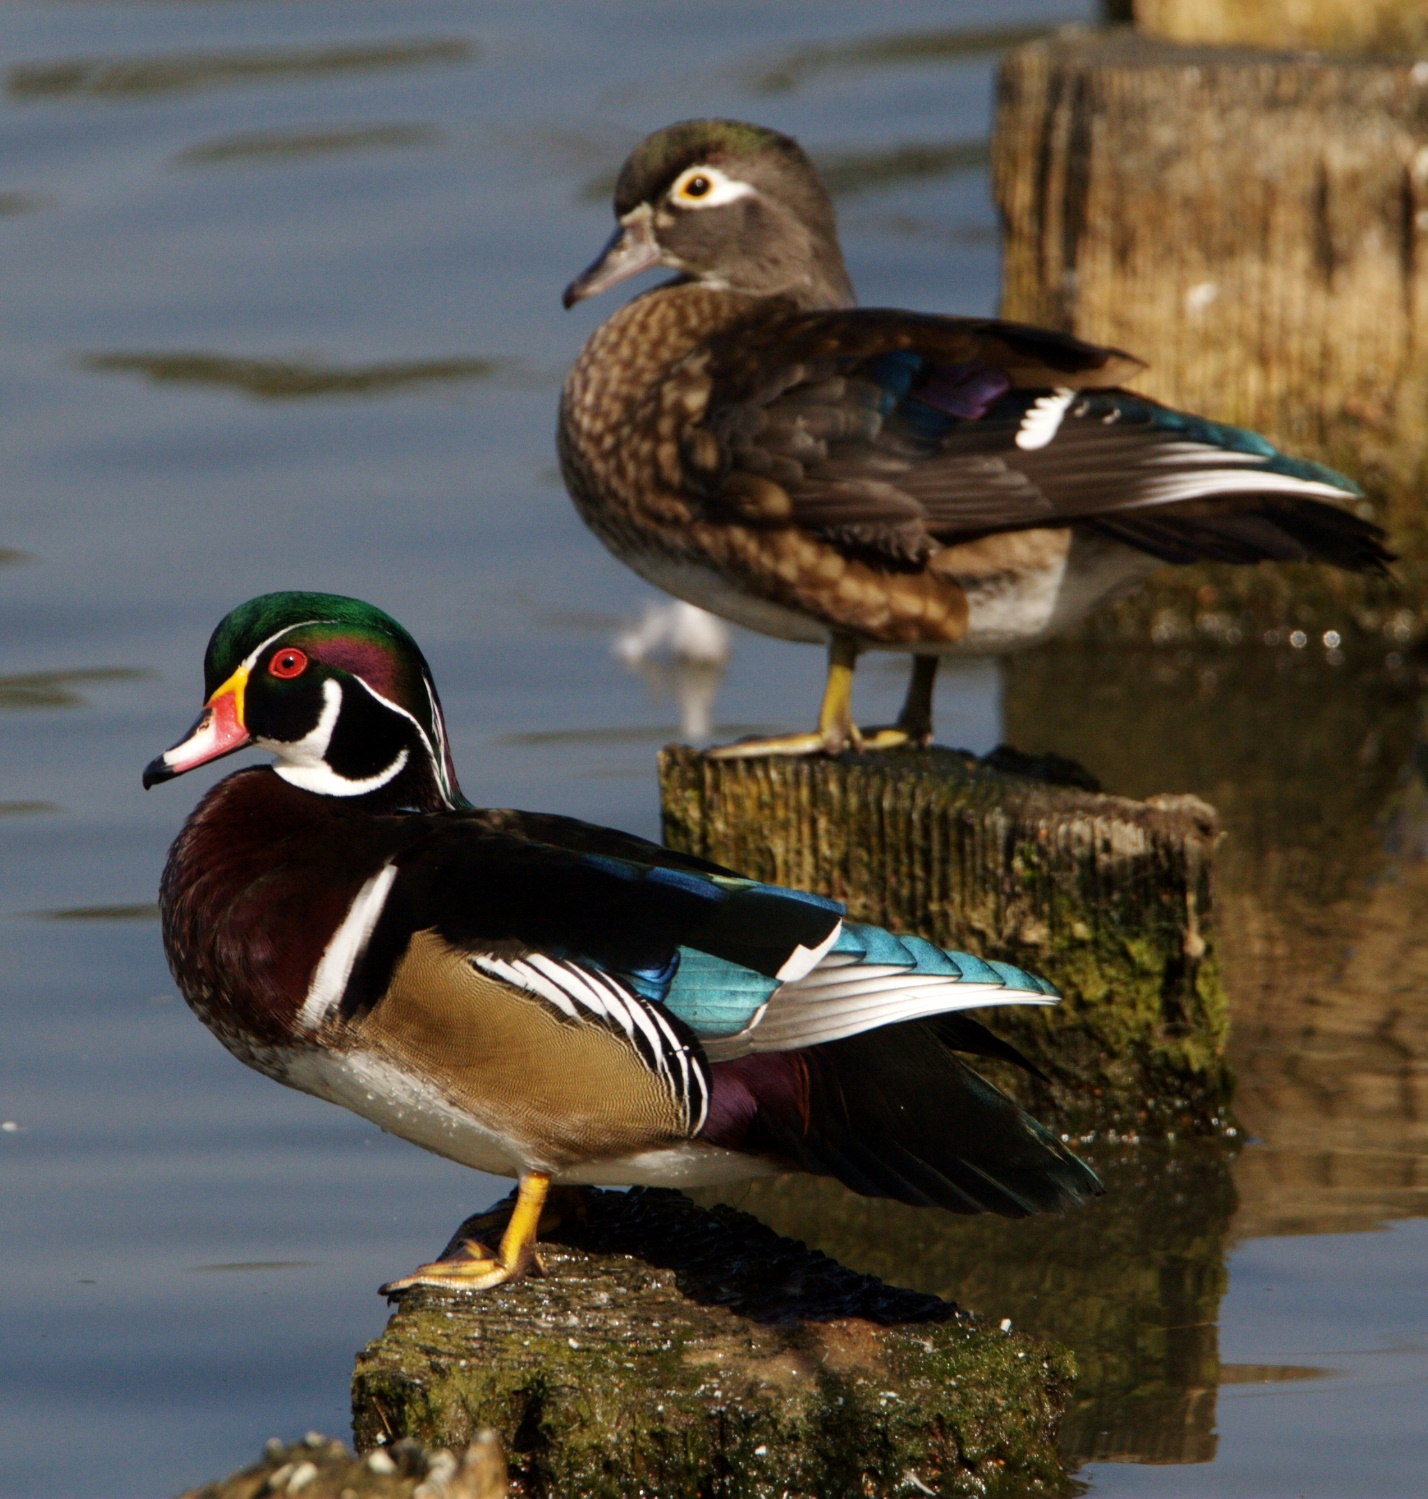
\includegraphics[width=\textwidth]{wood_duck_photo}
	\caption[Representative photo of Wood Duck]{Representative photo of Wood Duck drake (front) and hen (rear). Photo by Rick Leche – Photography, Flickr Creative Commons, \ccbyncnd{2.0} \url{https://www.flickr.com/photos/goellnitz/33597600618/}.}
	\label{fig:wood_duck_photo}
\end{figure}
\clearpage}
 

Like the Hooded Merganser, the Wood Duck constructs nests inside hollow tree cavities favoring similar habitat of swamps and sloughs with plentiful wooded cover, though they gravitate toward comparatively shallower areas (Bellrose et~al.~1964, Ryan et~al.~1998, Silvestro 2013). Wood Duck also courts early relative to other waterfowl beginning as early as September. Breeding pairs begin searching for nests in the early spring and have been observed to begin laying in early March (Armbruster 1982). Wood Duck lay an average of 12 eggs per clutch with numbers varying from 7 to 15 (Dugger and Fredrickson 1992, Semel and Sherman 1992). Wood Duck has also been shown to heavily utilize artificial nest boxes placed on the landscape to supplement natural cavities (Bellrose et~al.~1964, Scherpelz 1979, Ryan et~al.~1998).   

Nest boxes are man-made wooden boxes placed to mimic the natural tree cavities animals would use (Figure~\ref{fig:nest_box}). They do not have a standardized construction or system of placement, and often their location is chosen for ease of maintenance. Additionally, boxes are made in a variety of sizes with the entry hole regulating what species can access it. This results in those boxes used by Hooded Merganser and Wood Duck also being used by competing species such as Common Goldeneye \textit{(Bucephala clangula)}, owls, and potential predators such as racoons, snakes, and some woodpeckers (Heusmann and Stolarski 2017). It is unclear how the success of Hooded Merganser nests in boxes compare to those in natural cavities; research of other cavity-nesting bird species showed that different species had increased, similar, or decreased success in boxes compared to natural cavities (Purcell et~al.~1997).

\afterpage{%
\begin{figure}[p!]
	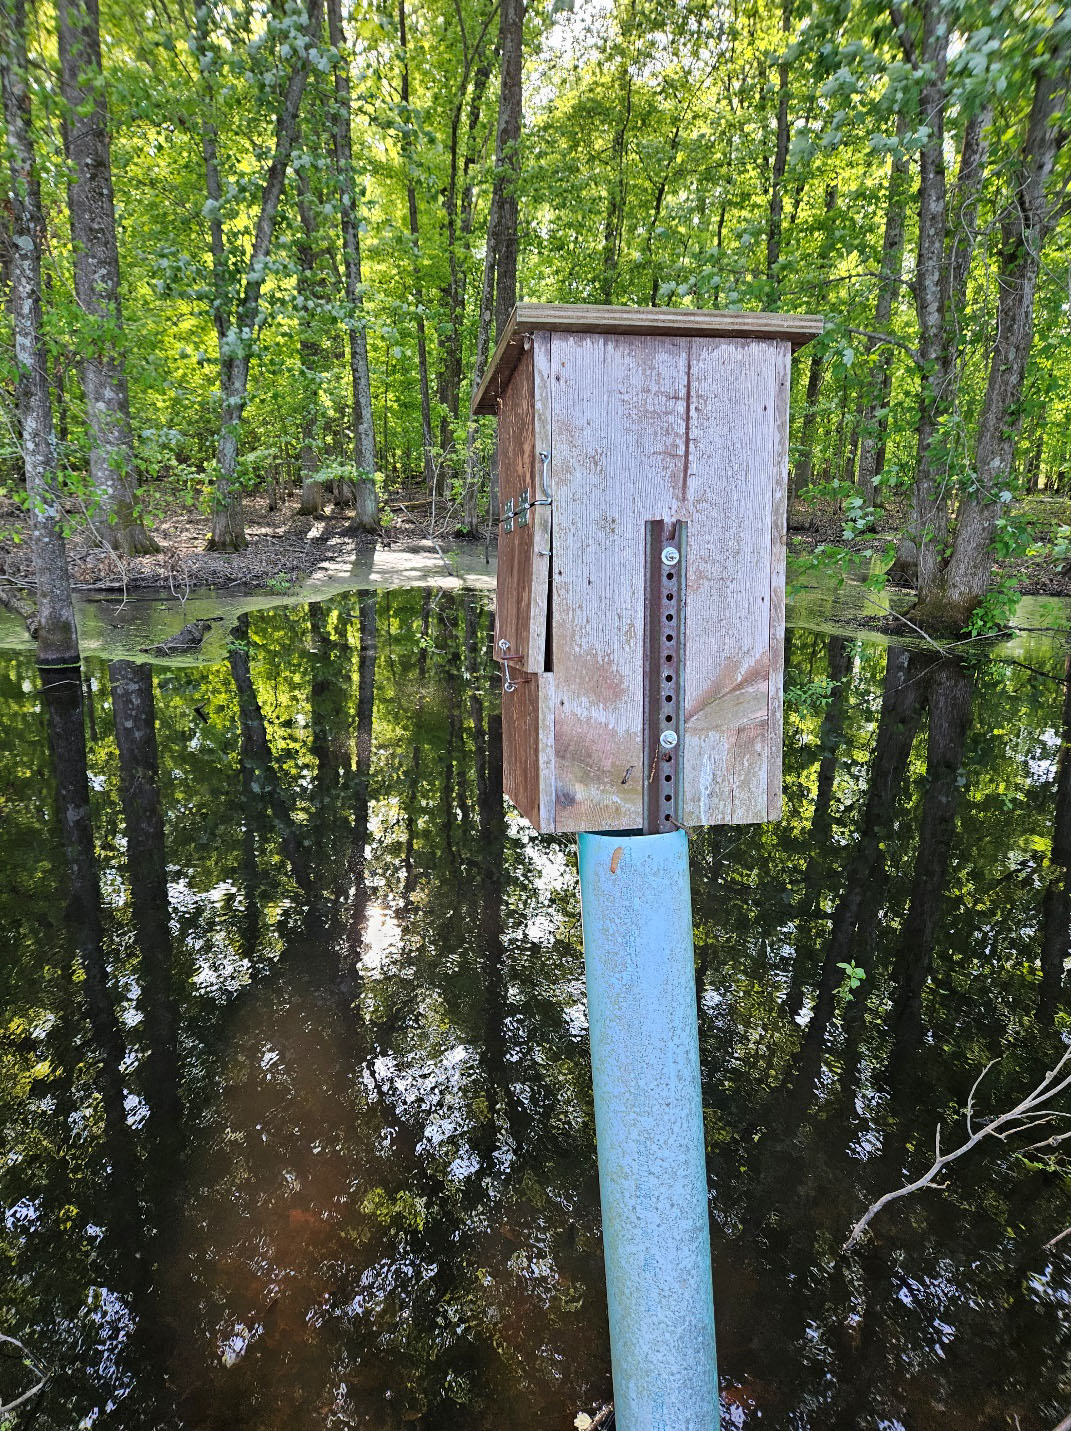
\includegraphics[height=0.85\textheight]{nest_box}
	\caption[Representative photograph of a nest box and surrounding habitat ]{Representative photograph of a nest box (S7) and surrounding habitat at Duck Creek Conservation Area, Puxico, Missouri. The door to access the nest is visible on the left side of the box. Photo by Frank J.~Irovic.}
	\label{fig:nest_box}
\end{figure}
\clearpage}
 


\section*{Prior research}

Nesting by the Hooded Merganser is little studied, usually in combination with other cavity-nesting species including Wood Duck (McNicol et~al.~1997, Mallory et~al.~2002). However, even these studies give valuable insight into merganser nesting. Previous studies have detailed general nesting behavior and success rates (Clawson et~al.~1979, Soulliere and Rusch 1996, Mallory et~al.~1998). Historical band-return data indicated that most mergansers returned to the same nesting locations each year, with 82\% of females nesting within one mile of their previous nest (Morse et~al.~1969). They initiated nesting in late February and mid-April with peak initiation occurring during March. They lay an average on one egg every 1.4–3 days, then line the nest with down and begin incubation. At the end of the approximately 28-day incubation period 80\% of Hooded Merganser nests studied successfully hatched young (Morse et~al.~1969, SénéChal et~al.~2008).  

One study (Ludt~2003) of 40 nest boxes on the same management area found nest box use increased from 21\% in 1994 to 33\% in 1998 but hatching success decreased from 90\% to 79\%. This may have been due to increased brood parasitism from 13\% to 75\% along with the increased nest box use (Ludt~2003). Nest success may also be negatively affected by dump nesting, a common form of brood parasitism that entails a female laying their eggs in another female’s nest. It is a common occurrence in birds with approximately 75 species making no nest and relying solely on dumping for reproduction (Hamilton and Orians 1965). Eggs dumped into Hooded Merganser nests may be from conspecifics or other species including Wood Duck and Common Goldeneye. Hens will displace dumped eggs to the periphery of the nest, potentially reducing their incubation efficiency (B. D. Dugger et~al.~1999).  In one study of Wood Duck, non-parasitized nests showed 78\% of eggs present hatched compared to only 63\% of eggs in parasitized nests (Clawson et~al.~1979). However, another study noted that despite similar negative effects on nest survival rates, interspecific brood parasitism minimally impacted Wood Duck breeding productivity (Bakner et~al.~2024). No comparable studies of the effects of dump nesting on Hooded Merganser have apparently been performed.

Additional research focused on the nest boxes themselves and their surrounding habitat. The use of nest boxes increased nest density compared to before box use. Nest boxes also increased the number of eggs per clutch, with the largest clutch increasing from 16 to 24 eggs from 1981–1985 (Zicus 1990).  Nest boxes might increase vulnerability to predation, which has been shown to impact up to 50\% of nests (Christman and Dhondt 1997, Pöysä et~al.~1997). Racoons successfully destroyed 43\% of Wood Duck nest boxes without predator guards but were unable to invade a single box (0\%) with predator guards (Lacki et~al.~1987). In contrast, the Black Rat Snake can circumvent predator guards to consume eggs and sometimes kill incubating Hooded Merganser hens (Fendley 1980).  


Few studies have addressed the habitat parameters that influence Hooded Merganser and Wood Duck choice among available nest boxes.  Hooded Merganser targets food sources by diving so they likely would favor deeper water, as it would allow for more efficient foraging while laying and incubating eggs. In contrast, the Wood Duck habit of foraging at or near the surface may make shallower water more advantageous for them. Due to foraging differences, I predicted that Hooded Merganser would use artificial nest boxes located near deep water but Wood Duck would favor shallower water. To test this prediction artificial nest boxes at Duck Creek Conservation Area in southeast Missouri were surveyed during the spring and summer of 2024.  Water width and tree coverage within 100 m\textsuperscript{2} were also measured because they might also influence nest box choice. 


	
\chapter{MATERIAL AND METHODS} % start of your main text
	%!TEX encoding = UTF-8 Unicode

\section*{Study area}

D\textsc{cca} is an intensively managed wetland located near Puxico, Missouri, managed by the Missouri Department of Conservation (\textsc{mdc}; Figure~\ref{fig:area_map}). The area totals 2,557 ha including a 728 ha shallow lake (Pool~1), 486 ha of actively managed bottomland hardwood forest (Pool~2 and Pool~3), and marsh units. The pool and forest areas provide habitat for Hooded Mergansers and Wood Ducks year around but particularly during their breeding season. The shallow lake known as Pool 1 serves as a large food source housing robust populations of fish and aquatic invertebrates. The bottomland hardwood forest provides nesting habitat and is seasonally flooded in the winter to provide roosting and foraging habitat. The area is bordered by the federally managed Mingo National Wildlife Refuge with another 8,500 ha of similar habitat.  Two other nearby \textsc{mdc} conservation areas, Ten Mile Pond and Otter Slough are managed in conjunction with \textsc{dcca} to provide wintering and spring nesting waterfowl habitat across southeastern Missouri. 

\afterpage{%
\begin{figure}[p!]
	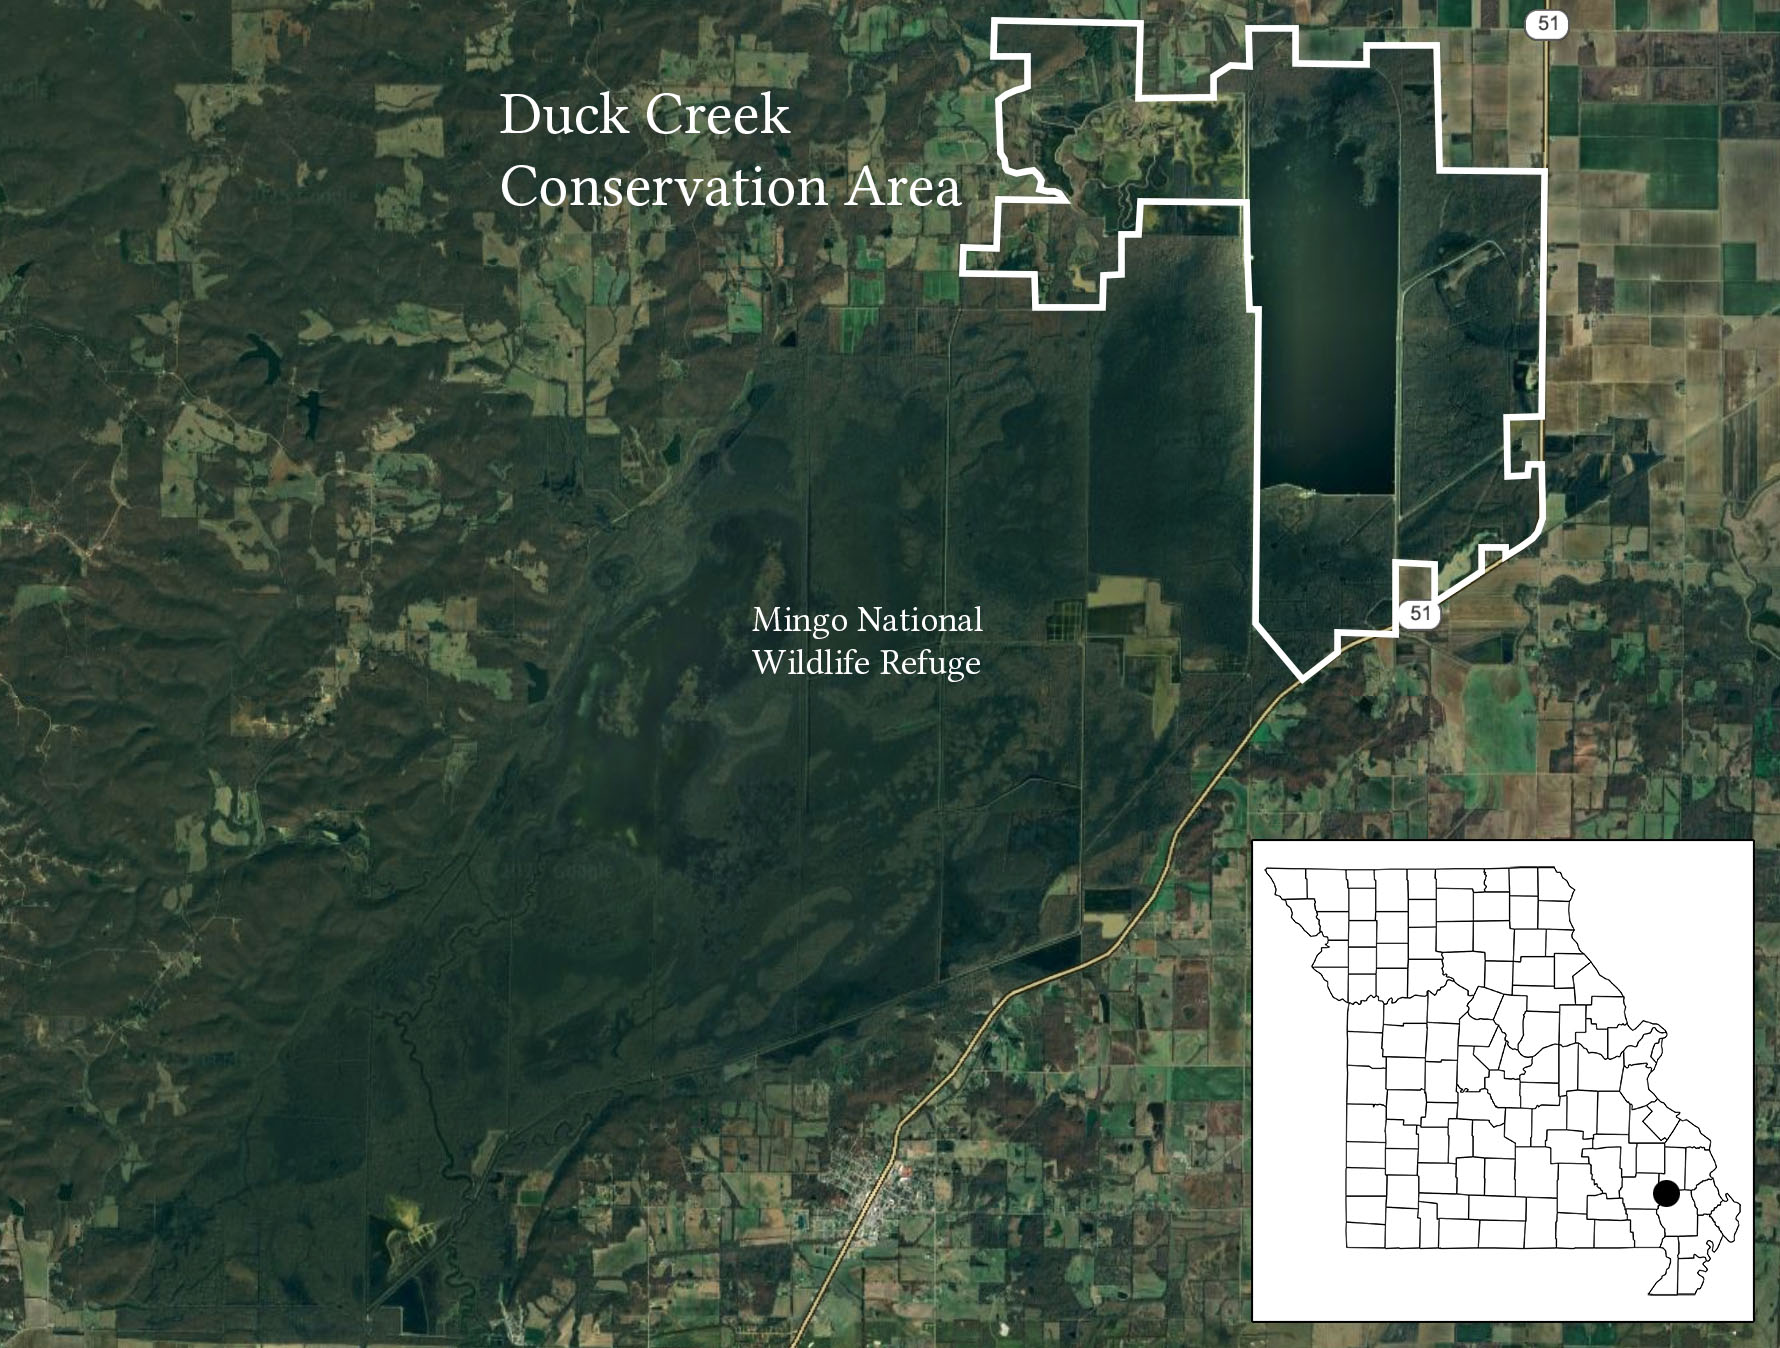
\includegraphics[width=\textwidth]{area_map}
	\caption[Duck Creek Conservation Area in southeast Missouri]{Duck Creek Conservation area and Mingo National Wildlife Refuge in Southeast Missouri. The approximate boundary of Duck Creek Conservation Area is outlined in white.}
	\label{fig:area_map}
\end{figure}
\clearpage}
 


\section*{Data collection}

The \textsc{mdc} maintains about 100 nest boxes for Hooded Merganser and Wood Duck reproduction, distributed around Pools 1–3.  Ten nest boxes were selected randomly from each pool for a total of 30 boxes to monitor hatching success (Figure~\ref{fig:nest_box_map}).  Pool~1  boxes were typically located along wider, deeper ditches with little tree cover. Pool~2 boxes were located along much narrower, shallower ditches with moderate tree cover. Pool~3 boxes were located on a mixture of broad flooded woods, narrow to wide ditches with heavy tree cover. For each box, tree cover and number of nearby boxes was measured using onXmaps GPS software (OnX Hunt 2025). Boxes were checked weekly from 23 March through 28 June 2024 to measure water width and depth, count eggs laid, hatched, abandoned, or lost, and identify both egg and nesting hen species. Weekly monitoring of nests ensured eggs were counted after hatching and to reduce the chance of eggshells being destroyed before counting. 

\afterpage{%
\begin{figure}[p!]
	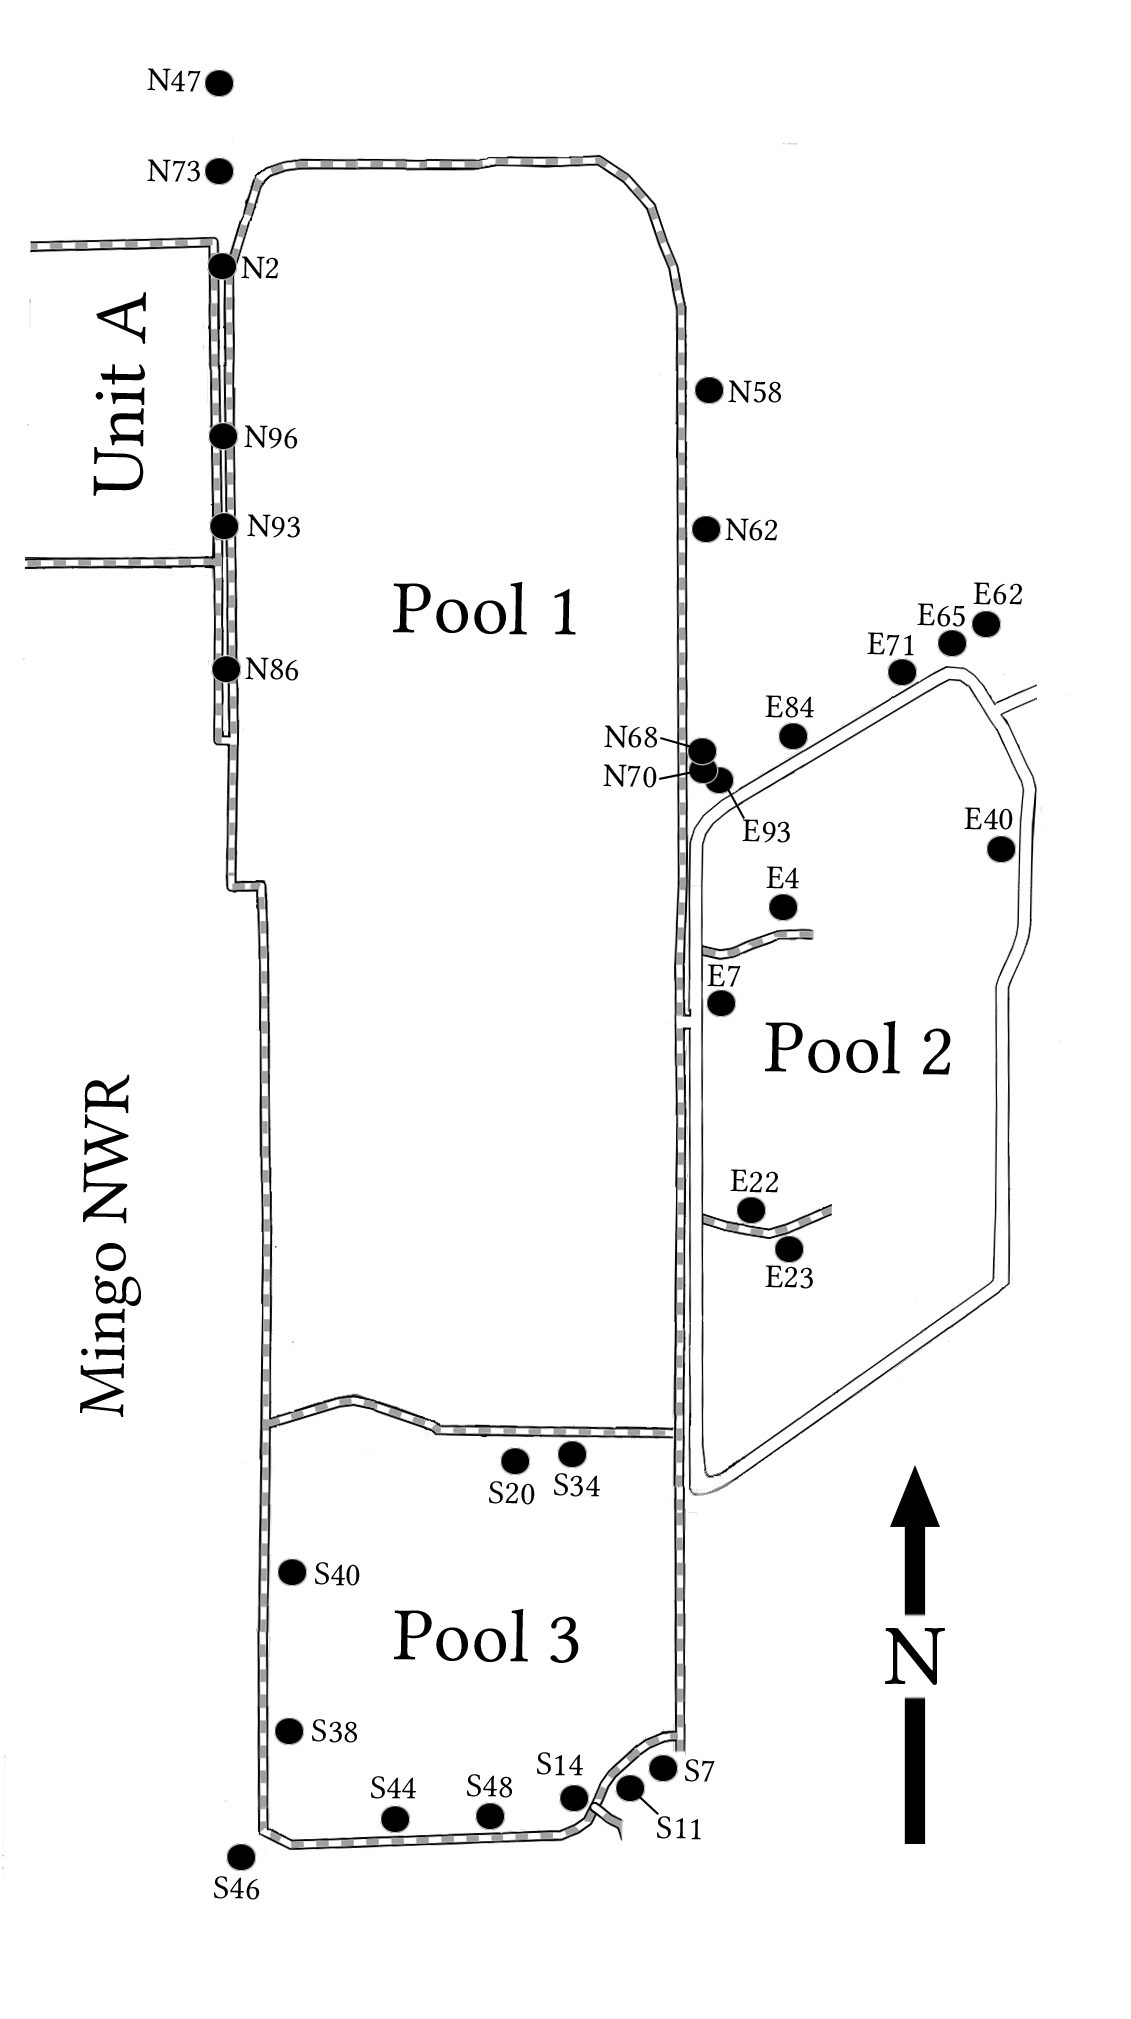
\includegraphics[height=0.85\textheight]{nest_box_map}
	\caption[Map showing location of 30 duck nest boxes sampled for this study]{Map showing location of 30 duck nest boxes sampled for this study. Boxes in the north section are located adjacent to Pool 1. Boxes in the east section are located adjacent to Pool 2. Boxes in the south section are located adjacent to Pool 3.}
	\label{fig:nest_box_map}
\end{figure}
\clearpage}
 

Dump nesting within and between species was determined by inspecting the size, shape, and color of eggs present. Wood Duck eggs are relatively small, tan to brown, and oblong. By comparison, Hooded Merganser eggs are larger, paler, and rounder (Figure~\ref{fig:wood_duck_nest}). Dump nesting by conspecifics was determined by additional eggs being counted at later inspections or by eggs lagging in development stage upon first inspection. Development stage was determined by egg candling, a process where a dark tube is used to observe light passing through an egg (Figure~~\ref{fig:candling_example}) to observe the embryo. The shape and position of the developing embryo can be used to estimate the age of the egg in days (Jalaludeen et al. 2022, Figure~\ref{fig:egg_candling}).  If an egg was developmentally behind others in the nest it was considered dumped. In nests with only Wood Duck eggs or where heterospecific dump nesting was present, two eggs were candled to establish the age of the nest. In nests with only Hooded Merganser eggs, eggs were candled until dump nesting was found or all eggs were candled. Wood Duck nests were not able to be fully candled and Hooded Merganser nests were stopped once dumping was found due to permit restrictions.  

\afterpage{%
\begin{figure}[p!]
	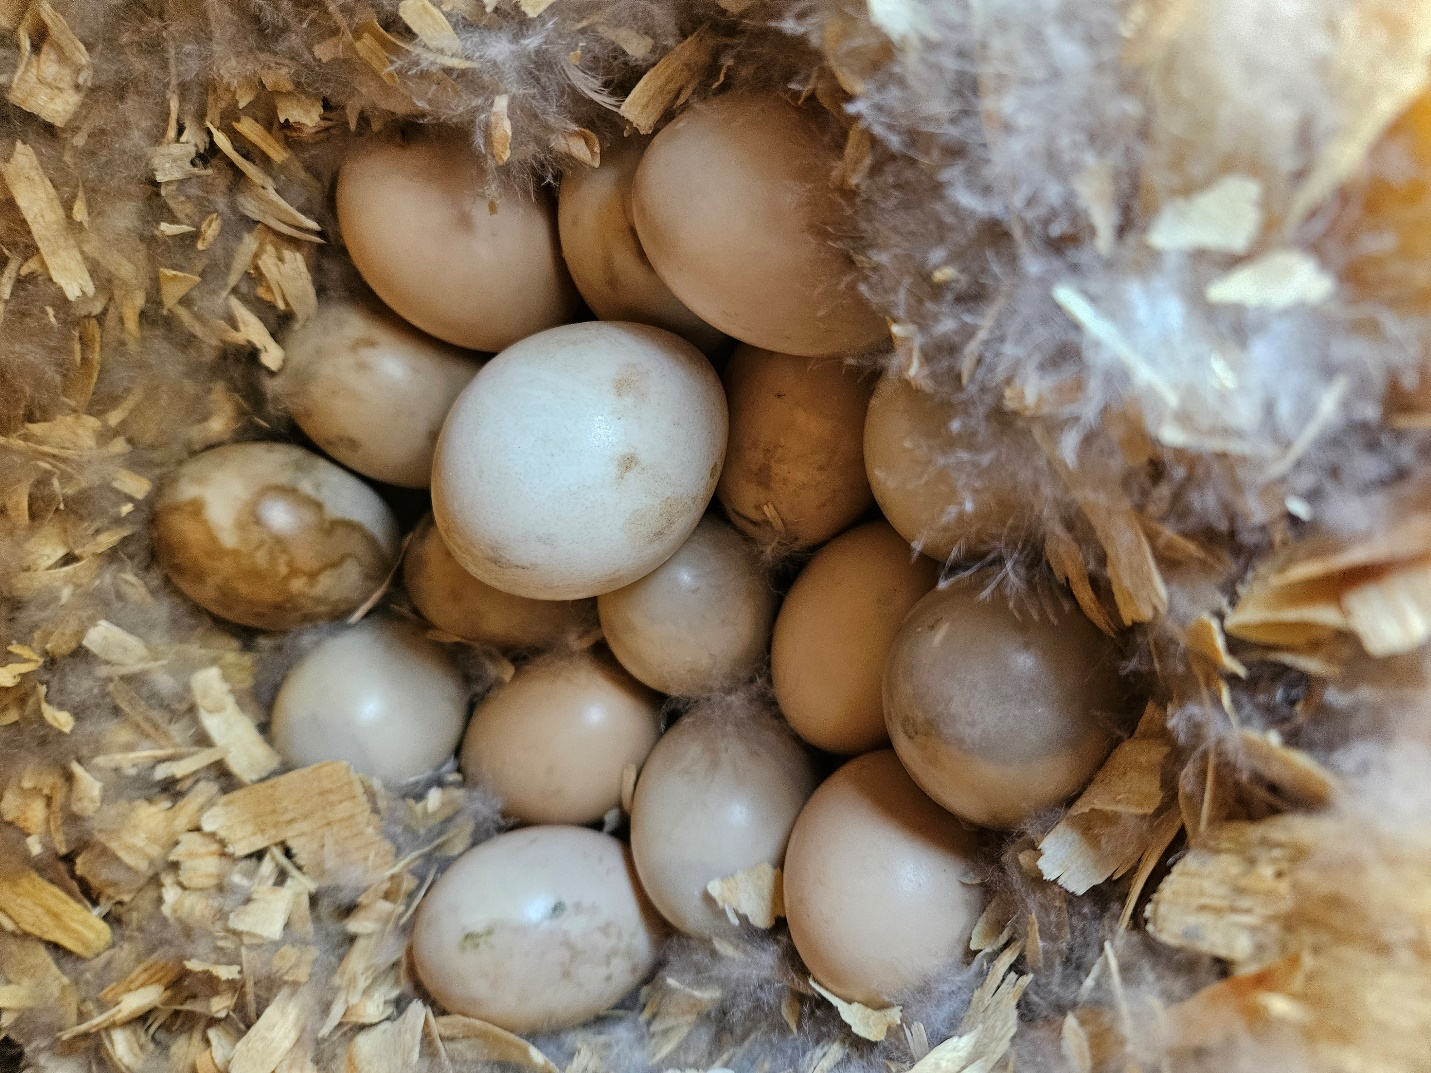
\includegraphics[width=\textwidth]{wood_duck_nest}
	\caption[Photograph of a Wood Duck nest with a dumped Hooded Merganser egg on top]{Photograph of a Wood Duck nest with a dumped Hooded Merganser egg on top in box E65 at Duck Creek Conservation Area, Puxico, Missouri. Wood duck eggs are visually smaller, browner, and more oblong where the Hooded Merganser egg is slightly larger, paler, and rounder by comparison. Photo by Frank J.\,Irovic. }
	\label{fig:wood_duck_nest}
\end{figure}
\clearpage}
 

\afterpage{%
\begin{figure}[p!]
	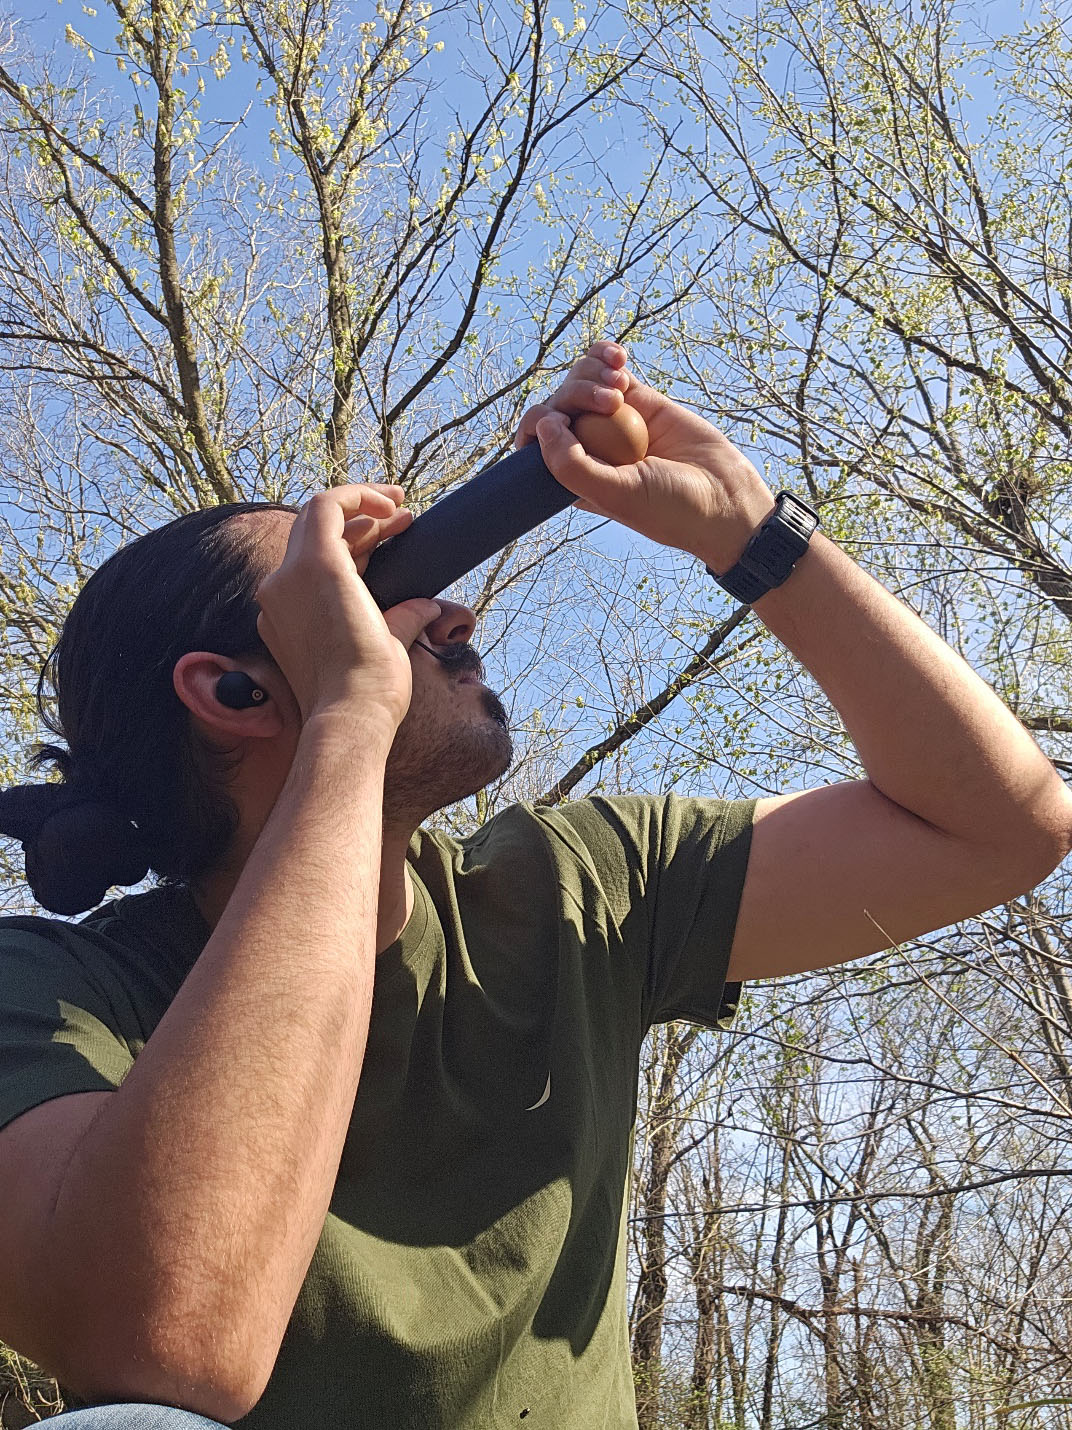
\includegraphics[width=0.99\textwidth]{candling_example}
	\caption[Photograph demonstrating a representation of egg candling]{Photograph demonstrating a representation of egg candling using a chicken egg. Photo by Frank J.~Irovic.}
	\label{fig:candling_example}
\end{figure}
\clearpage}
 

\afterpage{%
\begin{figure}[p!]
	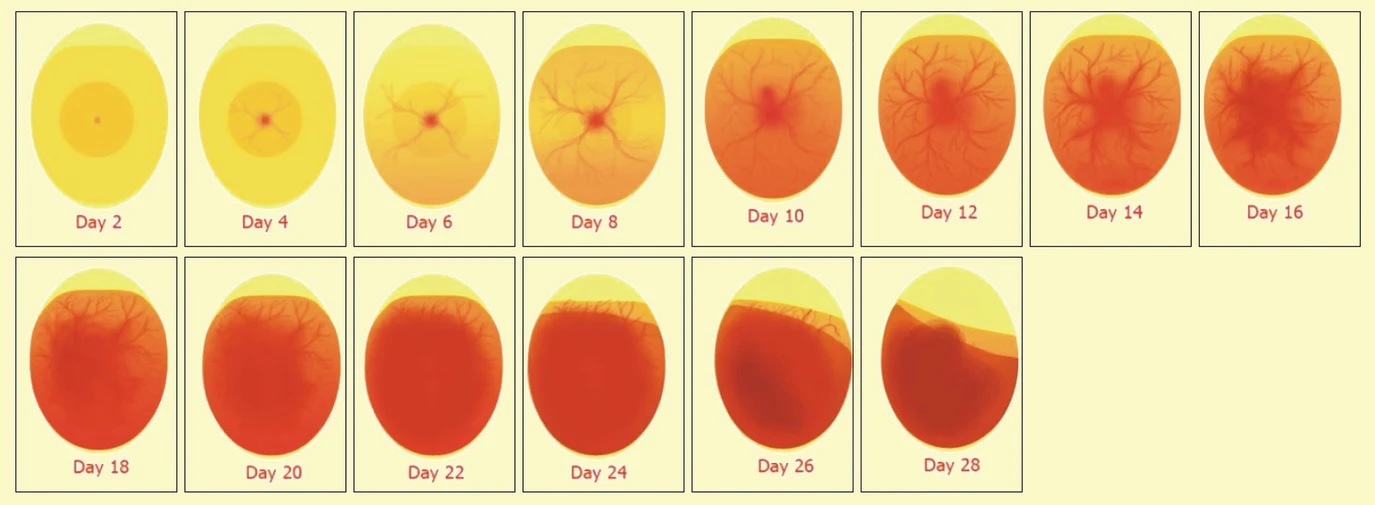
\includegraphics[width=\textwidth]{egg_candling}
	\caption[Developmental diagram of embryo development in ducks]{Developmental diagram of embryo development in ducks. Days indicate days since the start of incubation. Hatching occurs at approximately 28 to 29 days. Figure modified from Jalaludeen et~al.\,2022.}
	\label{fig:egg_candling}
\end{figure}
\clearpage}
 

At each weekly inspection, width and depth of water nearest the nest box was measured manually and the box was photographed. At the initial inspection of a nest its eggs would be identified, counted, and candled. Additionally, at the initial and all subsequent inspections eggs were counted to identify dumping or predation loss and the nests were photographed. This ensured that any changes to the nest could be confirmed in weekly intervals. Eggs were considered hatched, lost, or abandoned. Eggs that were present during the inspection prior to hatching were confirmed through counting eggshells after the nest was hatched. Any eggs that were found to have gone missing between weekly inspections were counted as lost to predation.  Any eggs that remained intact after the nest hatched were considered abandoned.  

\section*{Data analysis}

R statistical computing software version 4.4.1 (R Core Team 2024) was used for analysis. A\textsc{nova} or \textit{t}-tests from base R were used to test for significant differences of habitat variables among sections or egg-related variables (e.g. hatching) between species. If significant differences of habitat variables were identified among sections, then Tukey's Honestly Signficant Difference (\textsc{hsd}) test was used  for post-hoc determination of which sections were significantly different from the others. 

%A master dataset was compiled with all variables recorded for each of the thirty boxes. This was then edited down into an analysis dataset featuring box number, box section, species, number of eggs hatched, log of tree coverage, and the modal width and depth of the nearest water while the nest was active. Log of tree coverage was used as the values for coverage were significantly larger than the other variables resulting in points being clustered close together without visual separation. Log coverage in contrast maintained the relative distribution of points to each other while spreading them further apart. This allowed for a visually clearer figure and easier data interpretation. 

Non-metric multidimensional scaling \textsc{(nmds)} analysis was performed in R using the meta\textsc{mds} function from vegan 2.6-8 (Oksanen et al. 2025). N\textsc{mds} is an ordination technique that represents multiple variables on two to three axes while preserving the ordering of objects (e.g., nest boxes) along those variables (Rabinowitz 1975, Legendre and Legendre 1998). Bray-Curtis distance was used to estimate the ordering relationship among nest boxes based on number of eggs hatched, water width and depth, and tree coverage. Only data from nest boxes with attempted nesting events were used in the \textsc{nmds} analysis. 




\chapter{RESULTS}
	%!TEX encoding = UTF-8 Unicode

\section*{Habitat}

Water levels did not fluctuate much during the study (Figures~\ref{fig:water_width_plot} and~\ref{fig:water_depth_plot}), so  modal width and depth were used for analysis.  Water width was not significantly different among the pools ($F_{2,27} = 2.87, p = 0.074$; Figure~\ref{fig:water_width_plot}). Pool~2 was the narrowest ($\overline{x} =$ \num{5.3} \unit{\meter}). Pool~1 trended wider ($\overline{x} =$ 6.4 m). Pool~3 was much wider than the other  pools on average ($\overline{x} = 11.9$ \unit{\meter}) but this was due to boxes S20 and S34 (Figure~\ref{fig:nest_box_map}) that were located along a broad, shallow pool. Most other nest boxes in Pool~3 were along ditches with widths comparable to Pools~1 and~2  (Figure~\ref{fig:water_width_plot}). Water depth was significantly different among the 3 pools ($F_{2,27} = 4.77, p < 0.017$). Pool~1 was significantly deeper ($\overline{x} = 1.6$ \unit{\meter}) than Pool~2 ($\overline{x} = 0.56$~\unit{\meter}) and Pool~3 ($\overline{x} = 0.74$~\unit{\meter};  Table~\ref{tab:wd_hsd_table} and Figure~\ref{fig:hsd_wd_plot}, Appendix A). Nest boxes on the west side of Pool~1 were located along a deeper and somewhat wider ditch compared to boxes on the east side of Pool~1 (Figures~\ref{fig:nest_box_map} and~\ref{fig:water_depth_plot}).  

\afterpage{%
\begin{figure}[p!]
	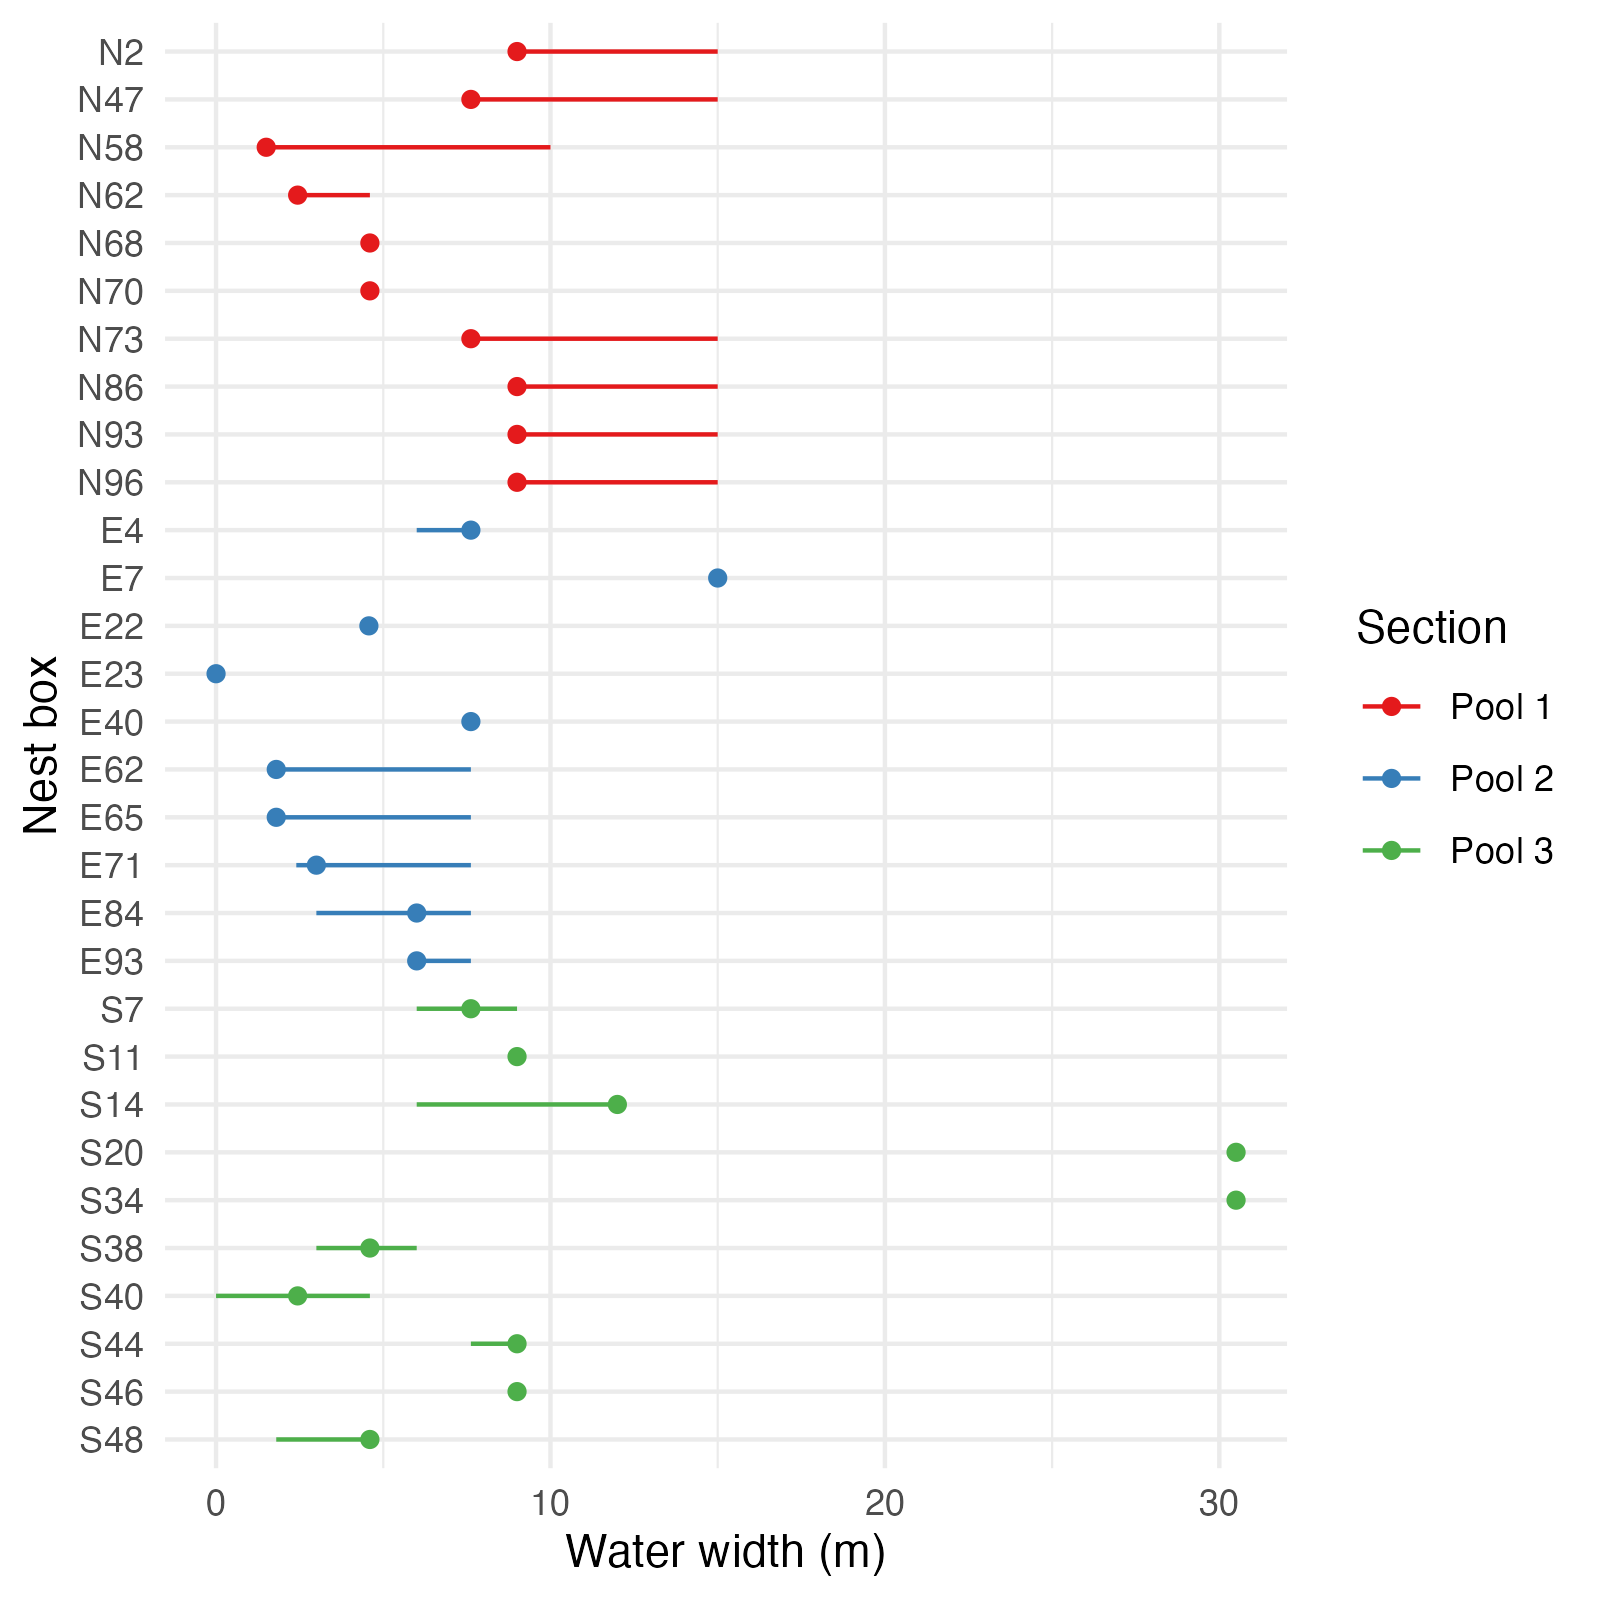
\includegraphics[width=\textwidth]{water_width_plot}
	\caption[Range and mode of water width measured for each nest box.]{Range and mode of water width measured weekly for each nest box during the study. Range is indicated by line segments. Mode is indicated by dots.}
	\label{fig:water_width_plot}
\end{figure}
\clearpage}


\afterpage{%
\begin{figure}[p!]
	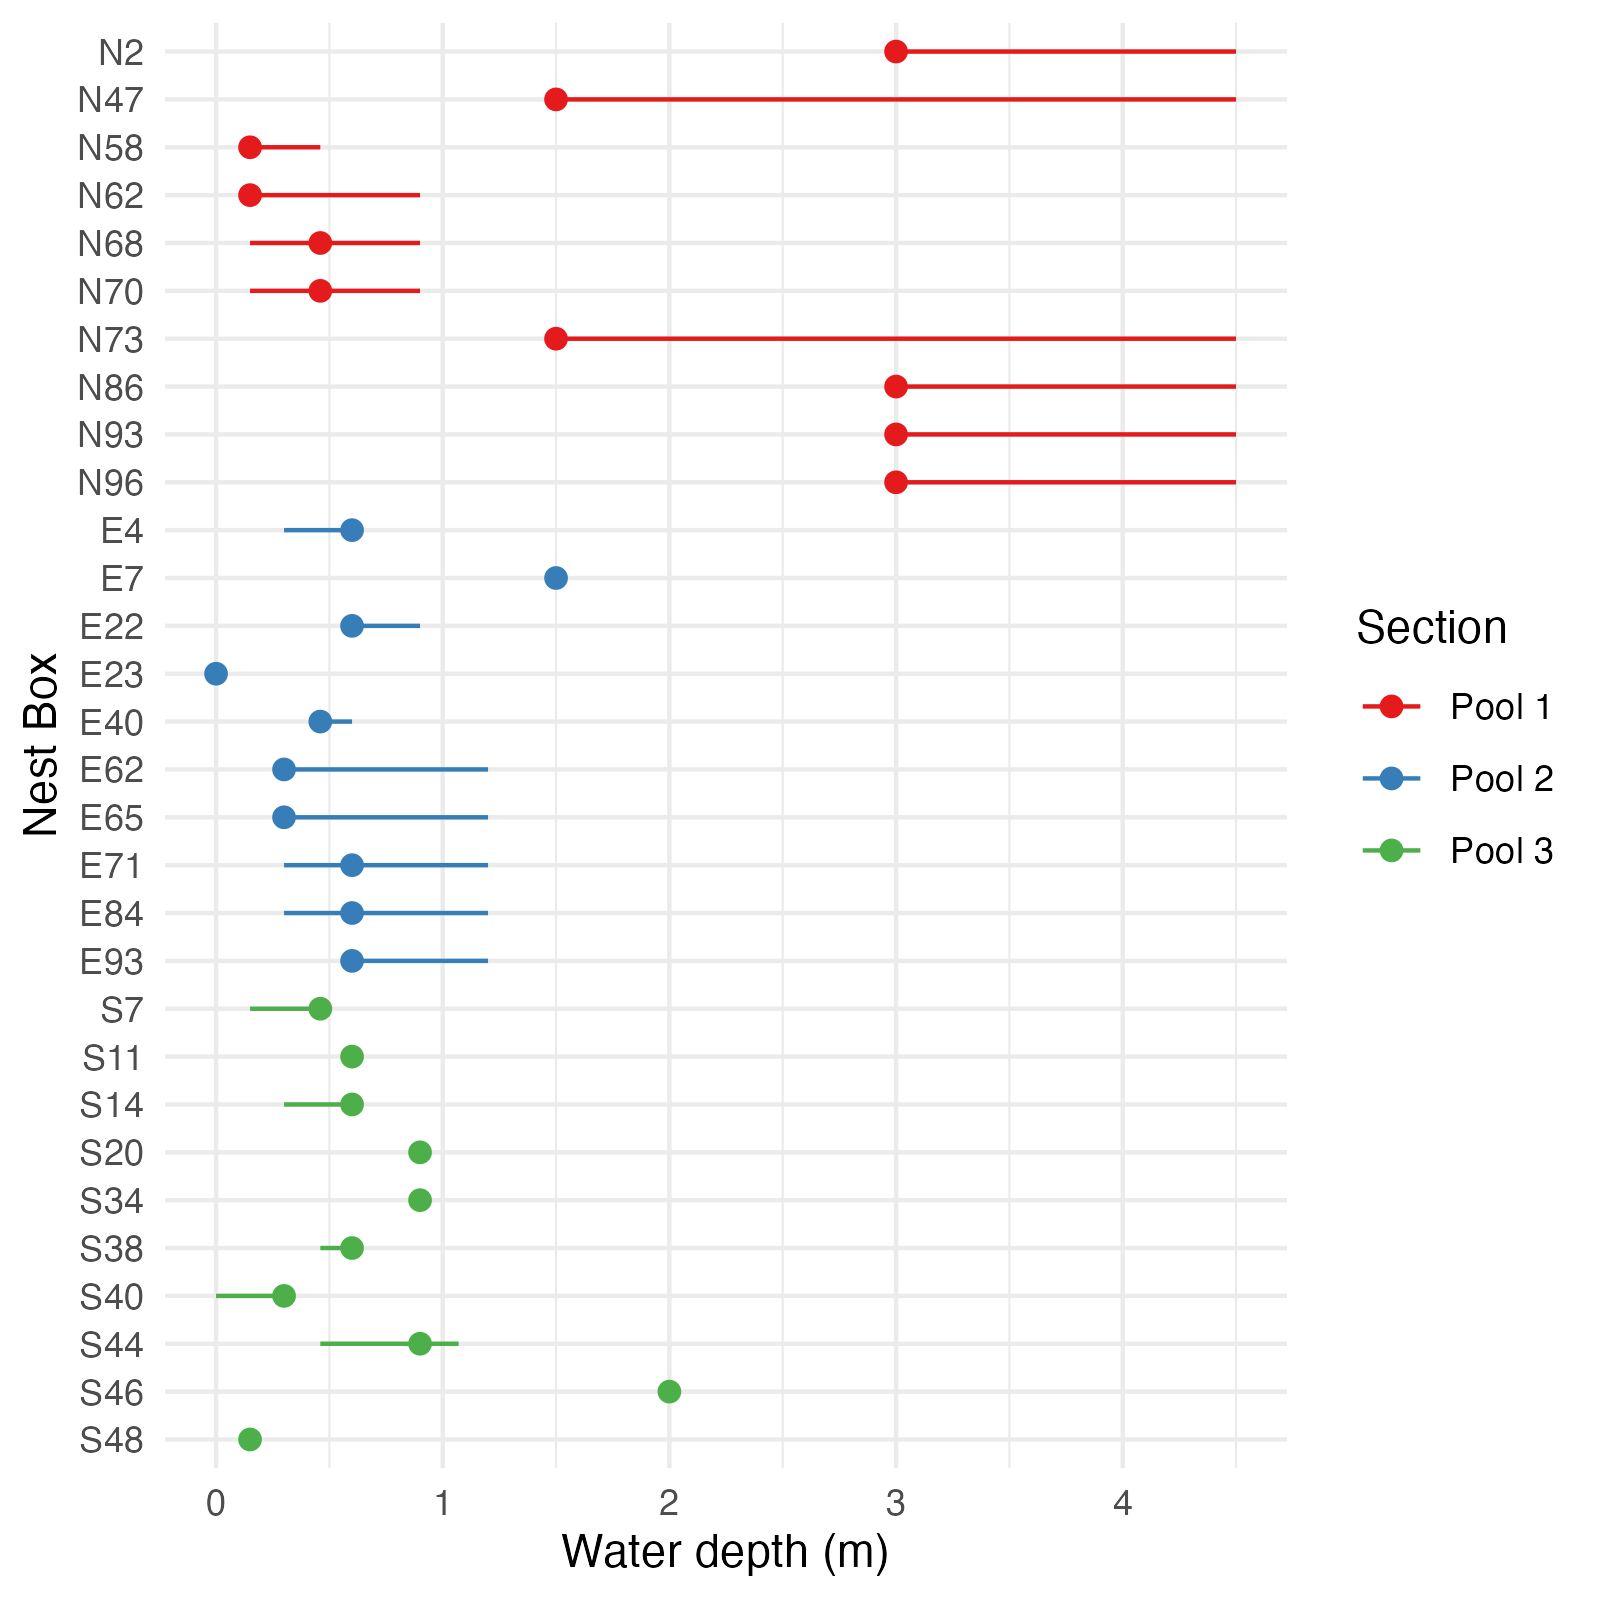
\includegraphics[width=\textwidth]{water_depth_plot}
	\caption[Range and mode of water depth measured for each nest box.]{Range and mode of water depth measured weekly for each nest box during the  study. Range is indicated by line segments. Mode is indicated by dots.}
	\label{fig:water_depth_plot}
\end{figure}
\clearpage}


Tree coverage differed significantly among the 3 pools ($F_{2,20} = 6.032, p < 0.009$; Table~\ref{tab:anova_coverage}; Figure~\ref{fig:tree_coverage_plot}). Pool~1 was significantly more open ($\overline{x} = 13{,}628$ \unit{\meter\squared}) compared to Pool~2 ($\overline{x} = 25{,}176$ \unit{\meter\squared}) and Pool~3 ($\overline{x} = 23{,}669$ \unit{\meter\squared}) (Table~\ref{tab:coverage_hsd_table} and Figure~\ref{fig:hsd_coverage_plot}, Appendix A), due to the proximity of the large and open areas of Pool~1 and Unit~A. 

\afterpage{%
%\begin{Spacing}{1}
\begin{table}
\addfontfeatures{Numbers=Monospaced}
\centering
\begin{threeparttable}
\caption[Analysis of variance results for amount of tree coverage]{Analysis of variance results for amount of tree coverage among the three pools in Duck Creek Conservation Area.}\label{tab:anova_coverage}
\noindent\begin{tabular}[l]{@{}lrrrrr@{}}
\toprule
Source of variation & $df$ & $SS$ & $MS$ & $F$ & $p$ \tabularnewline
\midrule
Pool & 2 & 381221000 & 190610500 & 6.032 & 0.00891 \tabularnewline
Residuals & 20 & 631951315 & 31597566 & & \tabularnewline
\bottomrule
\end{tabular}
\end{threeparttable}
\end{table}
%\end{Spacing}
\clearpage
}

\afterpage{%
\begin{figure}[p!]
	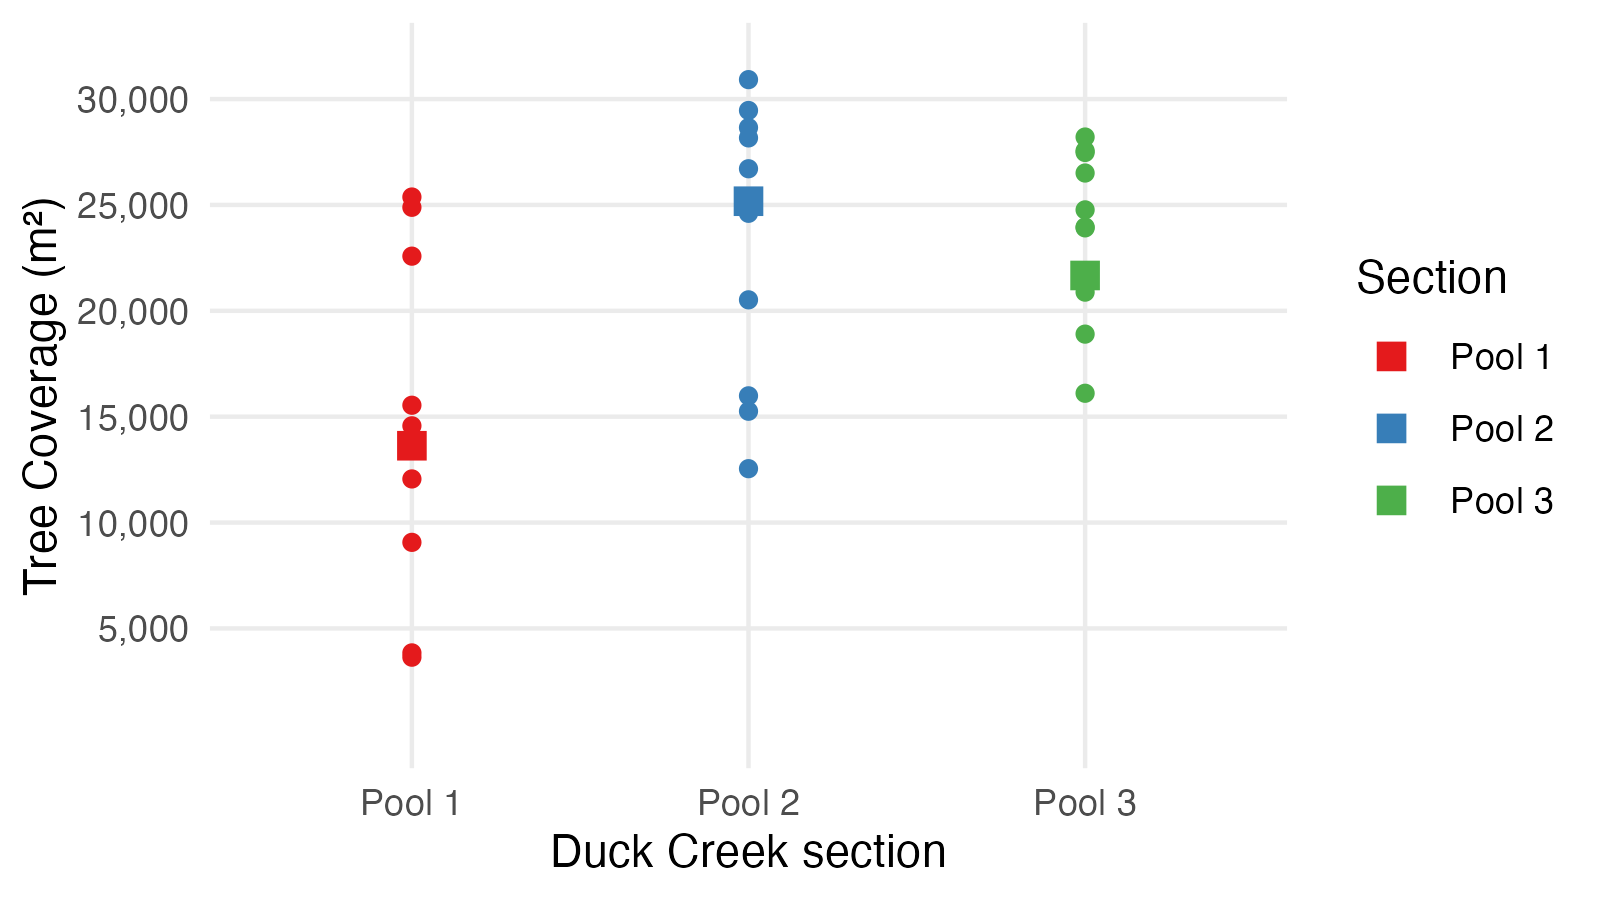
\includegraphics[width=\textwidth]{tree_coverage_plot}
	\caption[Range and mean of tree coverage]{Range and mean of tree coverage for each section. Dots indicate individual measurements. Triangle indicates mean coverage for each section.}
	\label{fig:tree_coverage_plot}
\end{figure}
\clearpage}


\section*{Nesting}

Nesting events occurred in 17 of the 30 nest boxes (56.7\%) during this study. A second, sequential nesting attempt occurred in 6 of the 17 boxes, for a total of 23 nests during the study period. The second attempts were treated as independent nesting events for analysis. 
Hooded Mergansers accounted for 9 nesting events and Wood Ducks accounted for the other 14 events (Tables~\ref{tab:hooded_merganser_data_table} and ~\ref{tab:wood_duck_data_table}).  Ten nesting events occurred in the Pool~2 in 7 boxes. Nine of the events were by Wood Ducks; only one was by Hooded Merganser. Nine nesting events occurred in the Pool~3 in 7 boxes. Five of the events were by from Hooded Mergansers and four were by Wood Ducks. Four nesting events occurred in Pool~1 in separate boxes. Three events were by Hooded Mergansers and only one by Wood Duck. %No nests were observed in natural cavities in the vicinity of these nest boxes.  

\afterpage{%
\begin{landscape}		
%\begin{Spacing}{1}
\begin{table}
\addfontfeatures{Numbers=Monospaced}
\centering
\begin{threeparttable}
\caption[Hooded Merganser data for boxes with nesting events]{Hooded Merganser data for boxes with nesting events. Original eggs were laid by the occupying hen. Dumped eggs were added by a different hen. Hatched, abandoned, and lost include original plus any dumped eggs. See Table~\ref{tab:raw_data_eggs} for detailed nesting results.} \label{tab:hooded_merganser_data_table}
\noindent\begin{tabular}[l]{@{}R{1.5cm}R{1.5cm}R{1.5cm}R{1.2cm}R{1.5cm}R{2.0cm}R{1cm}R{1.8cm}R{1.8cm}R{2.7cm}@{}}
\toprule
& \multicolumn{6}{c}{Number of Eggs} & \multicolumn{2}{c}{Water} & \tabularnewline
\cmidrule(rl){2-7} \cmidrule(rl){8-9}
Nest box & Original & Dumped & Total & Hatched & Abandoned & Lost & Depth (m) & Width (m) & Tree Cover (m²) \tabularnewline
\midrule
E40 & 11 & 0 & 11 & 11 & 0 & 0 & 0.46 & 7.62 & 29,461\tabularnewline
S34 & 9 & 0 & 9 & 0 & 9 & 0 & 0.9 & 30.5 & 18,899\tabularnewline
S34 & 9 & 0 & 9 & 0 & 9 & 0 & 0.9 & 30.5 & 18,899\tabularnewline
S7 & 2 & 10 & 12 & 11 & 1 & 0 & 0.46 & 7.62 & 16,106\tabularnewline
S11 & 10 & 0 & 10 & 10 & 0 & 0 & 0.6 & 9 & 27,559\tabularnewline
S44 & 11 & 2 & 13 & 11 & 2 & 0 & 0.9 & 9 & 27,478\tabularnewline
N93 & 20 & 2 & 22 & 18 & 2 & 2 & 4.5 & 15 & 3,642\tabularnewline
N2 & 16 & 0 & 16 & 16 & 0 & 0 & 4.5 & 15 & 12,060\tabularnewline
N47 & 8 & 0 & 8 & 8 & 0 & 0 & 1.5 & 7.62 & 25,374\tabularnewline\bottomrule
\end{tabular}
\end{threeparttable}
\end{table}
%\end{Spacing}
\end{landscape}
\clearpage
}



\afterpage{%
\begin{landscape}		
%\begin{Spacing}{1}
\begin{table}
\addfontfeatures{Numbers=Monospaced}
\centering
\begin{threeparttable}
\caption[Wood Duck data for boxes with nesting events]{Wood Duck data for boxes with nesting events. Original eggs were laid by the occupying hen. Dumped eggs were added by a different hen. Hatched, abandoned, and lost include original plus any dumped eggs. See Table~\ref{tab:raw_data_eggs} for detailed nesting results.} \label{tab:wood_duck_data_table}
\noindent\begin{tabular}[l]{@{}R{1.5cm}R{1.5cm}R{1.5cm}R{1.2cm}R{1.5cm}R{2.0cm}R{1cm}R{1.8cm}R{1.8cm}R{2.7cm}@{}}
\toprule
& \multicolumn{6}{c}{Number of Eggs} & \multicolumn{2}{c}{Water} & \tabularnewline
\cmidrule(rl){2-7} \cmidrule(rl){8-9}
Nest box & Original & Dumped & Total & Hatched & Abandoned & Lost & Depth (m) & Width (m) & Tree Cover (m²) \tabularnewline
\midrule
E62 & 10 & 3 & 13 & 10 & 3 & 0 & 0.3 & 1.8 & 28,166\tabularnewline
E62 & 8 & 5 & 13 & 12 & 0 & 1 & 0.3 & 2.4 & 28,166\tabularnewline
E65 & 17 & 1 & 17 & 16 & 0 & 1 & 0.3 & 3 & 24,605\tabularnewline
E93 & 9 & 0 & 9 & 9 & 0 & 0 & 0.9 & 6 & 20,518\tabularnewline
E93 & 2 & 0 & 2 & 0 & 0 & 2 & 1.2 & 7.62 & 20,518\tabularnewline
E4 & 14 & 0 & 14 & 0 & 6 & 8 & 0.6 & 7.62 & 30,918\tabularnewline
E7 & 9 & 1 & 10 & 9 & 1 & 0 & 1.5 & 15 & 15,985\tabularnewline
E22 & 8 & 4 & 12 & 8 & 4 & 0 & 0.6 & 4.57 & 26,709\tabularnewline
E22 & 14 & 0 & 14 & 0 & 0 & 14 & 0.9 & 4.57 & 26,709\tabularnewline
S20 & 13 & 6 & 19 & 13 & 6 & 0 & 0.9 & 30.5 & 20,882\tabularnewline
S20 & 17 & 4 & 21 & 15 & 4 & 2 & 0.9 & 30.5 & 20,882\tabularnewline
S7 & 13 & 3 & 16 & 13 & 1 & 2 & 0.46 & 9 & 16,106\tabularnewline
S14 & 19 & 2 & 21 & 13 & 1 & 7 & 0.6 & 12 & 28,207\tabularnewline
N70 & 2 & 4 & 6 & 2 & 4 & 0 & 0.15 & 4.6 & 13,436\tabularnewline\bottomrule
\end{tabular}
\end{threeparttable}
\end{table}
%\end{Spacing}
\end{landscape}
\clearpage
}



Nesting success was based on the number of hatched eggs, including dumped eggs. Hooded Merganser hatched \numrange[range-phrase = –]{0}{18}, with a mean of \num{8.3} eggs. Wood Duck hatched \numrange[range-phrase = –]{0}{16} eggs, with a mean of \num{9.3} eggs. The number of hatched eggs was not significantly different between species ($t = -0.388, p = 0.702$). A significant interaction effect for number of eggs hatched did occur between species and pool ($F_{2,18} = 5.96, p < 0.05$; Table~\ref{tab:anova_table}). Hooded Merganser hatched a total of 42 eggs in the Pool~1 in three events compared to 11 eggs in Pool~2  (1 event) and 32 eggs in Pool~3 (5 events, including 2 failed events; Table~\ref{tab:hooded_merganser_data_table}; Figure~\ref{fig:hatched_eggs_plot}). Wood Duck hatched 64 eggs in Pool~2 in 6 boxes (9 events, including 3 failed). %Three boxes were used for sequential events. The second attempts in boxes E22 and E93 both failed. 
Wood Duck hatched 54 eggs in Pool~3 across four events in three boxes. This species made only one attempt in Pool~1 and hatched just 2 eggs (Table~\ref{tab:wood_duck_data_table}; Figure~\ref{fig:hatched_eggs_plot}). 

\afterpage{%
%\begin{Spacing}{1}
\begin{table}
\addfontfeatures{Numbers=Monospaced}
\centering
\begin{threeparttable}
\caption[Analysis of variance results for number of hatched eggs by species and pool]{Analysis of variance results for number of hatched eggs by species and pool.}\label{tab:anova_table}
\noindent\begin{tabular}[l]{@{}lrrrrr@{}}
\toprule
Source of variation & $df$ & $SS$ & $MS$ & $F$ & $p$ \tabularnewline
\midrule
Species & 1 & 4.9 & 4.90 & 0.216 & 0.648 \tabularnewline
Pool & 2 & 37.4 & 18.71 & 0.824 & 0.455 \tabularnewline
Species * Section & 2 & 270.6 & 135.31 & 5.957 & 0.010 \tabularnewline
Residuals & 18 & 408.9 & 22.72 &  & \tabularnewline
\bottomrule
\end{tabular}
\end{threeparttable}
\end{table}
%\end{Spacing}
\clearpage
}

\afterpage{%
\begin{figure}[p!]
	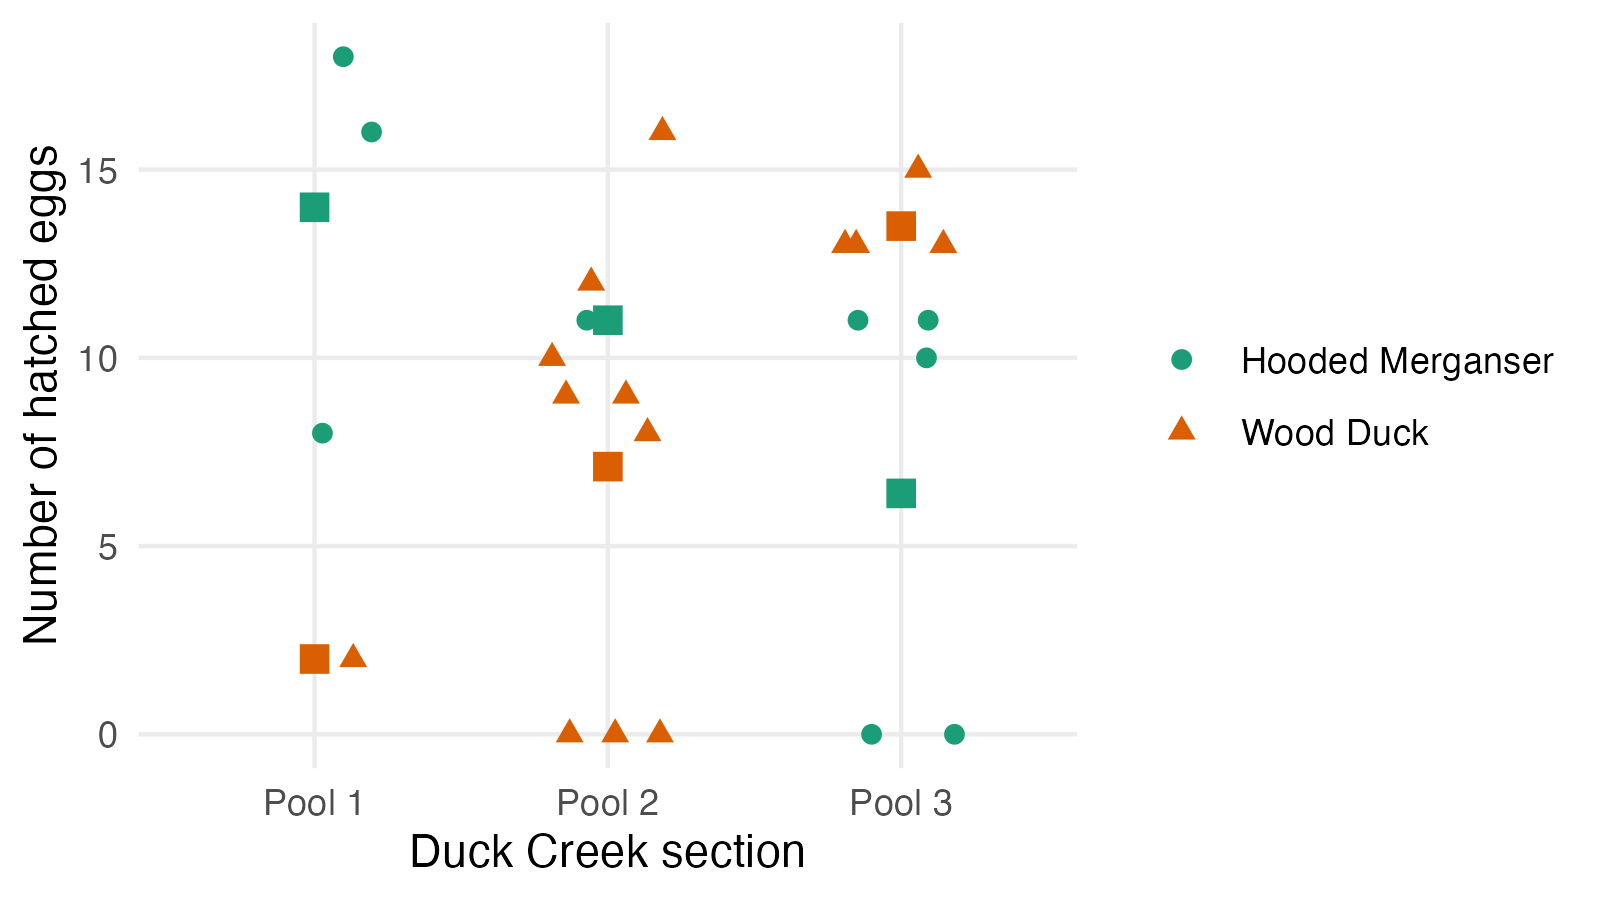
\includegraphics[width=\textwidth]{hatched_eggs_plot}
	\caption[Number of hatched eggs per nest box by pool]{Number of hatched eggs per nest box by pool. Green circles represent individual values for Hooded Merganser. Orange triangles represent individual values for Wood Duck. Green and orange squares represent mean number of eggs hatched in each pool for Hooded Merganser and Wood Duck, respectively. }
	\label{fig:hatched_eggs_plot}
\end{figure}
\clearpage}
 

Dump nesting was observed in 3 of 9 Hooded Merganser nests (Figure~\ref{fig:dumped_eggs_plot}). Egg dumping in Hooded Merganser nests occurred in nest boxes N93, S7, and S44, with 2, 2, and 10 eggs, respectively. These are the only three Hooded Merganser nests that did not have 100\% hatching success (Table~\ref{tab:hooded_merganser_data_table}). The most extreme dump nesting event for a Hooded Merganser hen was in nest box S7. The original hen laid only 2 eggs. An additional 10 eggs were added by Wood Duck. Only one Hooded Merganser egg hatched. The second was abandoned. All 10 Wood Duck eggs hatched (Table~\ref{tab:raw_data_eggs}, Appendix A). This was the only observed event where Wood Duck dump-nested in a Hooded Merganser nest.

In comparison, dump nesting occurred in 10 of 14 Wood Duck nests. The number of eggs dumped in Wood Duck nests ranged from 1–6, with a mean of 3.3 eggs. Only boxes E65, S20 attempt 2, and S14 saw fewer eggs hatched than those originally laid by the Wood Duck hen. Box E65 was the only observed instance of a Hooded Merganser egg being nest-dumped in a Wood Duck nest. For most cases, the number of eggs hatch in a nest with known dump-nesting, the number of eggs hatched matched the number of eggs laid originally by the Wood Duck hen.


\afterpage{%
\begin{figure}[p!]
	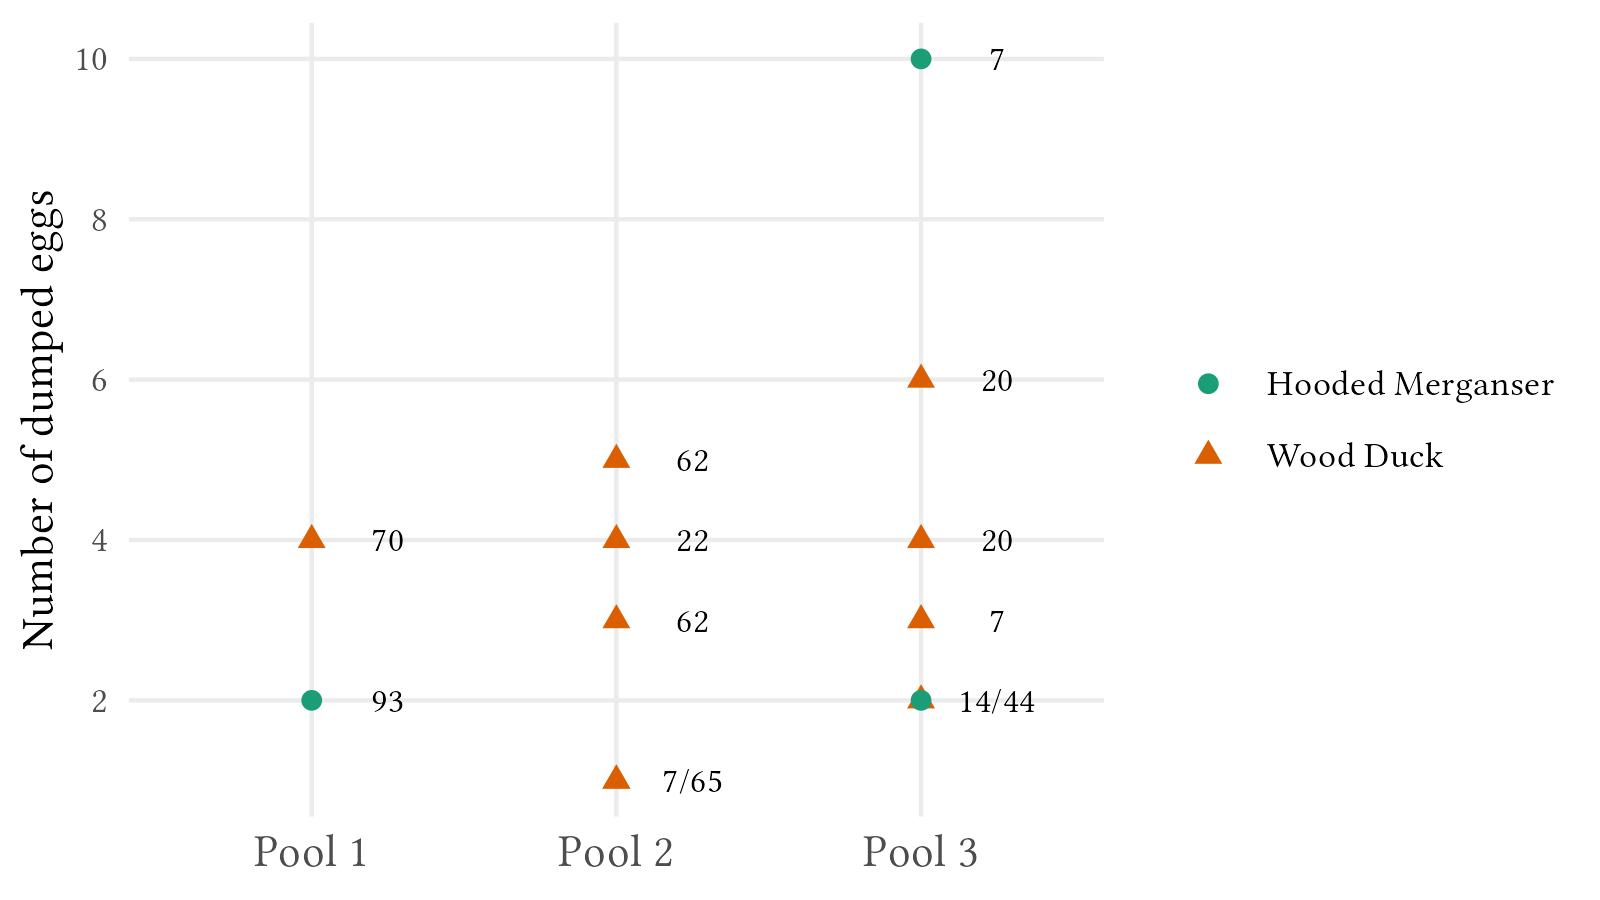
\includegraphics[width = \textwidth]{dumped_eggs_plot}
	\caption[Nest boxes with evidence of egg dumping]
	{Nest boxes with evidence of egg dumping for each pool of the study. Green circles indicate boxes with Hooded Merganser as the host species. Orange triangles indicate boxes with Wood Duck as the host species. Boxes N7 and N65 both had one egg dumped. Boxes S14 and S14 both had two eggs dumped. Box E62 had sequential nesting events, both by Wood Duck. Box S7 had sequential nesting events, first by Hooded Merganser followed by Wood Duck.}
	\label{fig:dumped_eggs_plot}
\end{figure}
\clearpage}
 


The relationship among hatching, water width and depth, and tree coverage was revealed by the \textsc{nmds} analysis (Figures~\ref{fig:nmds_plot_axes12} and~\ref{fig:nmds_plot_axes23}).  Both species had successful hatching for most nests (Figures~\ref{fig:nmds_plot_axes12} and~\ref{fig:hatched_eggs_plot}). Three Hooded Merganser nests were on the west side of the North section, which tended to have deeper water (Figures~\ref{fig:water_depth_plot} and~\ref{fig:nmds_plot_axes23}). Hooded Merganser had their highest number of eggs hatched in Pool~1 with nest boxes N2 and N93 (Figures~\ref{fig:hatched_eggs_plot} and~\ref{fig:nmds_plot_axes12}) although fewer eggs were hatched in nest box N47. Hooded Merganser did have success in Pool~2 and Pool~3. Two failed nests for Hooded Merganser were in Pool~3, both in box S34. 

\afterpage{%
\begin{figure}[p!]
	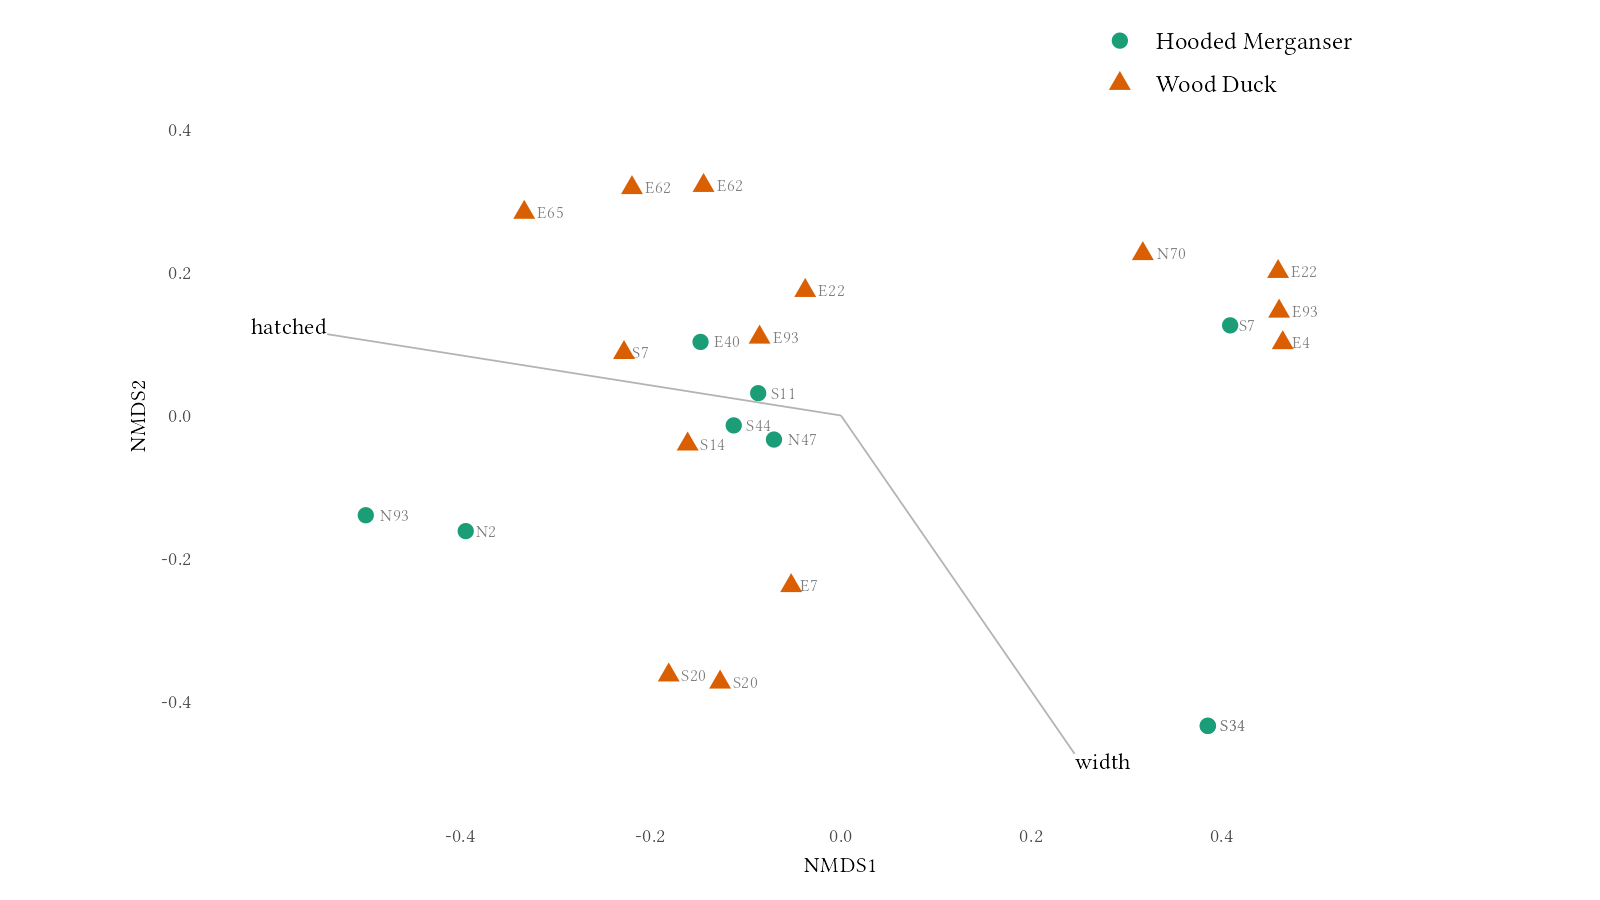
\includegraphics[width=\textwidth]{nmds_plot_axes12}
	\caption[N\textsc{mds} plot of axes 1 and 2]{Non-metric multidimensional analysis plot of axes 1 and 2. Green circles indicate nest boxes with Hooded Merganser as the original species. Orange triangles indicate nest boxes with Wood Duck as the original species. Light gray numbers show box~\textsc{id} numbers. N = Pool~1; E = Pool~2, S = Pool~3. Hatched and width variables provided the greatest rank-order separation on axis~1 and axis~2, respectively. Boxes to the left of the plot had greater numbers of hatched eggs. Boxes toward the lower half of the plot were associated with wider water. Stress = 0.023.}
	\label{fig:nmds_plot_axes12}
\end{figure}
\clearpage}
 

\afterpage{%
\begin{figure}[p!]
	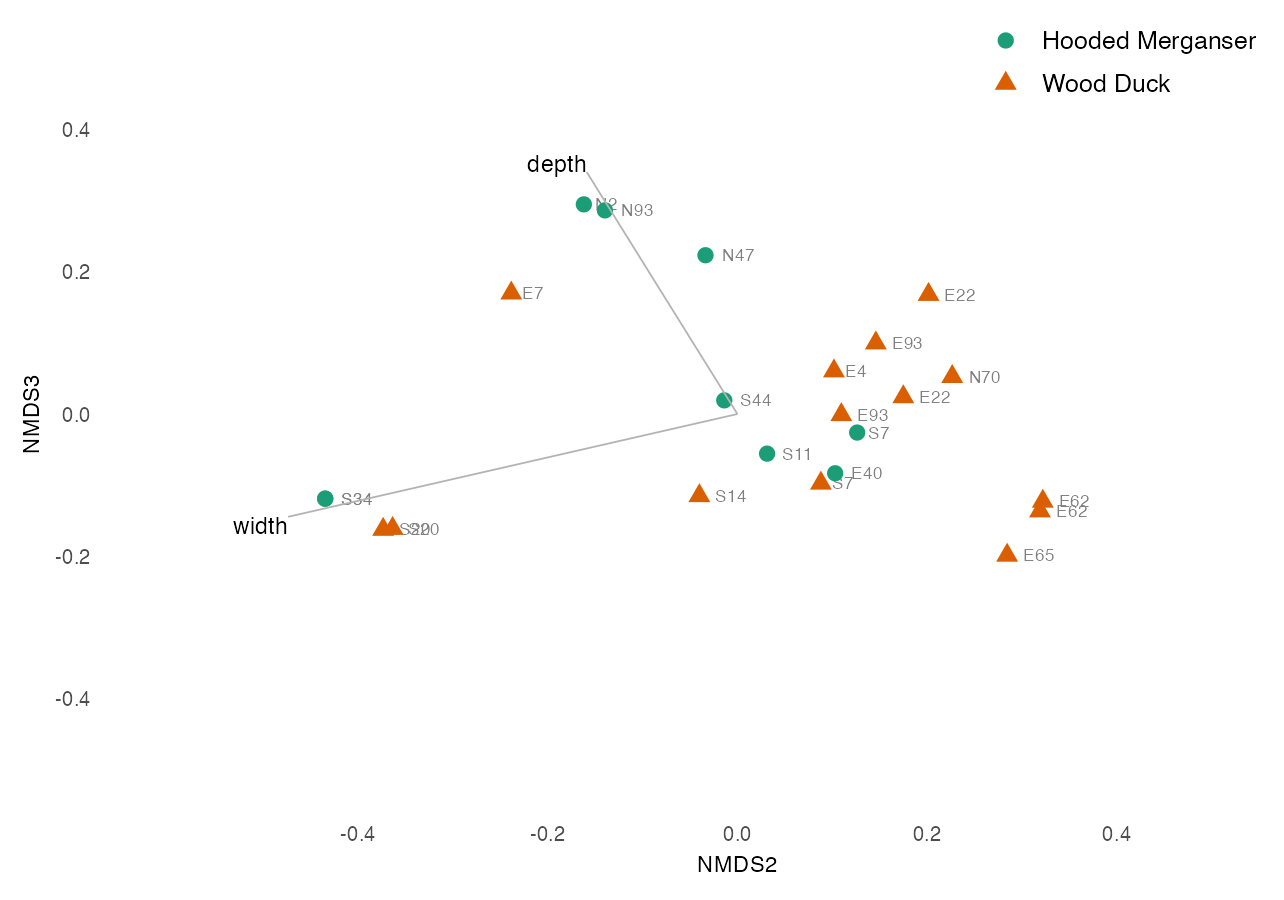
\includegraphics[width=\textwidth]{nmds_plot_axes23}
	\caption[N\textsc{mds} plot of axes 2 and 3]{N\textsc{mds} plot of axes 2 and 3.  Stress = 0.023.}
	\label{fig:nmds_plot_axes23}
\end{figure}
\clearpage}
 

Wood Duck nested mostly along the relatively shallow, narrow ditches (Figure~\ref{fig:nmds_plot_axes12}) of Pool~2 and Pool~3. They established only one nest on the east side of Pool~1 where the ditch is relatively shallow and narrow. Wood Duck did have two sequential nesting attempts in Pool~3 in the nest box S20, which is located along a broad, shallow pool. Wood Duck had two failed attempts in Pool~3 in nest boxes E4 and E93 (Figures~\ref{fig:hatched_eggs_plot} and~\ref{fig:nmds_plot_axes12}). %N\textsc{mds} stress was \num{0.023}, indicating a very good fit between the data and ordination results.




\chapter{DISCUSSION}
	%!TEX encoding = UTF-8 Unicode

Duck Creek Conservation Area includes three large pools as part of their waterfowl management program. Pool~1 includes a large reservoir that is mostly open but includes some bottomland hardwood forest at the northern end. Nest boxes were located along two long drainage ditches bordering the large reservoir. The ditch on the west side of Pool~1 is generally wider and deeper than that on the east side (Figure~\ref{fig:water_width_plot}) because this segment is located upstream of a major water control structure used to manage water levels throughout \textsc{dcca}. Overall, water depth adjacent to nest boxes of Pool~1 was significantly greater than the other pools. The north end of Pool~1 is also adjacent to Unit~A, a large open tract of wet meadows and small pools. The open areas of Pool~1 and Unit~A, combined with the wider west ditch, created significantly less tree cover than the other pools (Table~\ref{tab:anova_coverage}; Figure~\ref{fig:tree_coverage_plot}). Pool~2 is divided between some open water (flooded marsh and agricultural field) and a large tract of bottomland wood, with boxes located inside both habitats.  This pool tends to dry out due to water management practices for the area but the nest boxes are located along ditches or low spots in the woods that tend to retain water (Figures~\ref{fig:nest_box_map} and~\ref{fig:water_depth_plot}).  Pool~3 is almost entirely bottomland woods, with greater variation of water depth (less so for width) across the pool. Nest boxes in this pool are located adjacent to multiple flooded ditches of various widths, wide flooded woods, and a small pond. Despite this variability, mean water width and depth were similar between Pools~2 and~3 (Figures~\ref{fig:water_width_plot} and~\ref{fig:water_depth_plot}) as was tree coverage (Figure~\ref{fig:tree_coverage_plot}). 

Habitat variation across pools may influence nest box choice of Hooded Merganser and Wood Duck. Most Hooded Merganser nests were in Pool~1 (3 nests) or Pool~3 (5 nests). This species used only one nest box in Pool~2. The lone Hooded Merganser nest in Pool~2 was in an isolated box located on a slightly deeper and wider depression, separate from the ditch where most boxes were located. Hooded Merganser had their greatest hatching success in Pool~1, where all 3 nests were located on the deeper west ditch. Twenty original eggs plus 2 dumped eggs were laid in nest box N93 and 18 of themhatched.  Sixteen original eggs were laid in N2 and all hatched (Table~\ref{tab:hooded_merganser_data_table}).  Most often, Hooded Merganser hatched between 8–11 eggs. Two nesting attempts in the South section failed, both in box S34. Interestingly, 9 eggs were laid for each attempt, but the nest was apparently abandoned each time. Overall Hooded Merganser nested in boxes adjacent to water from 0.6–4.5 m deep, with those in Pool~1 being the deepest. Hooded Merganser may prefer nest boxes near deeper water because their diving and sight-pursuit foraging strategy requires water deep enough to allow diving and swimming for larger macroinvertebrates (Salyer and Lagler 1940, K. M. Dugger et~al.~1999).  

Wood Ducks nested most often in Pool~2 (9 nests) or Pool~3 (4 nests) but their mean hatching success was higher in Pool~3 ($\overline{x} = 7.1~\mathrm{vs.} 13.5$; Table~\ref{tab:wood_duck_data_table}).  A single Wood Duck nested on the east side of Pool~1 (box N70) adjacent to boxes in Pool~2 (Figure~\ref{fig:nest_box_map}). The ditch on the north side of Pool~2 flows into the ditch on the east side of Pool~1 at approximately the location of N70. Thus, the habitat of N70 is more like Pool~2 boxes than boxes on the west side of Pool~1. Overall, Wood Duck nests were adjacent to water 0.15–1.5 m deep.   



Wood Ducks may prefer nest boxes near shallower water due to their foraging habit. Wood Ducks either surface feed or dabble (Dugger and Fredrickson 1992) and therefore can only reach food sources as far as they can reach from the surface (Foth et~al.~2014). Although Wood Ducks of both sexes consume emergent and floating vegetation and seeds (Landers et~al.~1977) but invertebrates compose most of the breeding female’s diet to provide protein during egg production (Drobney and Fredrickson 1979). These food sources would be found either emergent in shallow water or along the edge of the shore, regardless of maximum water depth. Although Pools 2 and 3 were similar in terms of width and depth of the ditches adjacent to the nest boxes, as well as coverage, Pool~3 had far greater surface water area (personal observation) that could be used by Wood Ducks for foraging. Flooded forests may average higher invertebrate biomass compared to other wetland habitats (Hagy and Kaminski 2012 , Foth et~al.~2014). The comparatively higher amount of flooded forest in Pool~3 therefore may provide better foraging for breeding Wood Duck hens, resulting in higher success.  

Dump nesting did not appear to affect the hatch rate of originally laid eggs. Hooded Merganser nests saw varying success with 4 of the 9 nests hatching all eggs laid. Two other nests, both in S34, failed with none of their eggs hatched. After the original nest was abandoned, a new hen added additional nesting material to cover up the original clutch, and then laid her own eggs. As the new hen covered the previous eggs, this was considered a new nesting event instead of dump nesting. The three remaining nests hatched most of their eggs at 91.7\% (S7), 84.6\% (S44), and 81.8\% (N93) hatched respectively. These three were the only Hooded Merganser nests that saw dump nesting during this study (Figure~\ref{fig:dumped_eggs_plot}). In most cases, the dumped eggs were found abandoned, likely due to eggs being dumped after incubation and development of the other eggs had begun. Only S7 saw heterospecific dump nesting with 2 Hooded Merganser eggs and 10 Wood Duck eggs being dumped. A Hooded Merganser hen was observed leaving the nest box before most inspection, suggesting that she was the original hen.  

Wood Ducks in contrast saw only 1 of 14 nests hatch all eggs. Three nests, E4, E22 attempt 2, and E93 attempt 2, failed with no eggs hatched. The rest of the nests had variable hatch rates ranging between 33.4–92.3\%, but most hatch rates fell between 60–80\%. Similar to the Hooded Merganser nests all Wood Duck nests with a partial hatch rate were observed to have been dump nested (Figure~\ref{fig:dumped_eggs_plot}). The nest in box E65 experienced heterospecific dump nesting where all other instances were intraspecific. Similar to Hooded Merganser the abandoned eggs were generally those that were dumped. Prior studies have suggested that dump nesting can have negative, minimal, or positive effects on nest hatch rates and overall duckling recruitment (Clawson et~al.~1979, Eadie et~al.~1988, Bakner et~al.~2024). For example, conspecific dump nesting by waterfowl might be advantageous in some cases when driven by low resource availability or K-type life history (Eadie et~al.~1988).  This study did not address resource availability but the results do suggest that dump nesting is not always a successful reproductive strategy for the dumping hen, as most dumped eggs were left abandoned. 



\section*{Management implications}

Nest box placement relative to water proximity, entrance orientation, and box heights have been historically studied for Wood Ducks, as has natural cavity use and food selection during breeding (Bellrose et~al.~1964, Drobney and Fredrickson 1979, Lacki et~al.~1987, Ryan et~al.~1998). Nest box use by Hooded Mergansers has been less studied (Zicus 1990, Heusmann and Stolarski 2017), hindering consistent management of nest boxes when both species are present. When Hooded Mergansers are present, providing nest boxes adjacent to deeper water might enhance nest box use by this species. Wood Ducks were more likely to use nest boxes adjacent to shallower water. This difference gives wildlife managers at places such as DCCA another variable to consider that might support populations of both species directly and effectively. Further, most ditches at DCCA are shallower than the Pool~1 west ditch. Increasing the number or length of deeper ditches could provide more locations to increase the number of nest boxes that appeal to Hooded Merganser. The deeper ditches must also provide a suitable foraging base for this diving species. Further, this apparent preference for different water depths may also allow for management strategies to be applied across larger public and private areas. This may include one-time management strategies such as altering topography to increase the depth of ditches where nest boxes may be placed. Then, annually variable strategies such as installing water control structures may allow for yearly alterations in water characteristics and increase depth variation to support both Hooded Merganser and Wood Duck.  

Water depth may be an important habitat variable to consider for nest box placement, but these results must be interpreted cautiously. Only 17 boxes of 30 selected were used by Hooded Merganser and Wood Duck. Repeated nest attempts increased the total nesting events to 23 but only for a single nesting season. The small number of nest boxes studied may have resulted in incomplete knowledge of nest box use by each species. For example, a total of 13 nest boxes are located along the wide ditch on the west side of the North section (MDC, unpublished data). Six of these were selected at random for this study but only 3 were used by Hooded Merganser (and none by Wood Duck). Hooded Merganser had their highest nesting success in 2 of these boxes. However, it is unknown if additional nests were in any of the 7 other boxes along the west ditch of Pool~1 during this study. If additional nests were present in any of these boxes, the data here may represent a biased view of nest box use or hatching success. 

A more extensive data set may better reveal contributions for the variables measured here. For example, 9 Wood Duck nests and 1 Hooded Merganser nest were found across Pool~2. While Pool~2 was a mixture of open and wooded areas 33 of 43 boxes were in areas greatly to fully surrounded by cover. Of the 10 boxes included in this study, 8 were located in the heavily wooded areas. In contrast, the other 2 boxes were in more open areas and did not house nests during the study but the data but whether this can be explained by coverage, another variable, or randomness cannot be determined. Finally, the results obtained here might be explained by other variables not measured, such as box height or distance to nearest water (Lacki et~al.~1987). 

Dump nesting should also be considered as part of a comprehensive management program. In many cases, such as dump nesting in Wood Duck nests E62 attempt 1, E22 attempt 1, and S20, the dumped eggs were the eggs that did not hatch. In other cases, such as S20 attempt 2, and S14, the total number of hatched eggs was less than the number of eggs laid by the original hen. Reduced hatching success cannot be directly attributed to dump nesting but these data suggest that this behavior can reduce hatch success of both species. In addition, the actual rate of dump nesting could be underestimated. Fewer eggs could be candled in Wood Duck nests due to federal permit restrictions. In both species, conspecific eggs could only be determined by lagging development in candling or by eggs being abandoned. Eggs dumped prior to the start of incubation by a conspecific individual would develop at the same rate as non-dumped eggs so could not be distinguished. Regardless of these issues, the presence of Hooded Merganser and Wood Duck together with many available nest boxes provides an opportunity to study this behavior in greater detail.  

Nest boxes are an artificial alternative to natural tree cavities used by Hooded Merganser and Wood Duck. Variables in naturally occurring tree cavities such as tree species, cavity height, and cavity depth may be compared to further understand the natural reproductive behaviors and success of these species (Ryan et~al.~1998). Nest success can also be compared between natural tree cavities and artificial nest boxes to better understand how cavity and box use may influence nesting success (Bellrose et~al.~1964).  

Finally, other study methods could be used to compare new measurements, such as stress of the nesting hen, against nesting success. Corticosterone has been used as a measure of physiological stress in birds (Bortolotti et~al.~2008, Romero and Fairhurst 2016, Johns et~al.~2018). Blood corticosterone has recently been used to measure handling stress in captive Wood Ducks (Broadus et~al.~2025). Thus, blood corticosterone levels might be useful to assess stress levels in wild ducks like Wood Ducks and Hooded Mergansers.  


 
 \backmatter
 
\OnehalfSpacing

 \chapter{LITERATURE CITED}
	%!TEX encoding = UTF-8 Unicode

\begin{hangparas}{2em}{1}
	
	Armbruster, J.\,S. 1982. Wood Duck displays and pairing chronology. The Auk 99:116–122. 
	
	Bakner, D.\,L., K.\,M.\,Ringelman, and L.\,A.\,Reynolds. 2024. Wood duck nest survival and duckling recruitment is minimally affected by interspecific brood parasitism from Hooded Mergansers and Black-bellied Whistling-ducks. PLoS ONE 19:e0305899. 
	
	Bellrose, F.\,C., K.\,L.\,Johnson, and T.\,U.\,Meyers. 1964. Relative value of natural cavities and nesting houses for Wood Ducks. Journal of Wildlife Management 28:661. 
	
	Bortolotti, G.\,R., T.\,A.\,Marchant, J.\,Blas, and T.\,German. 2008. Corticosterone in feathers is a long-term, integrated measure of avian stress physiology. Functional Ecology 22:494–500. 
	
	Brasher, M.\,G., J.\,J.\,Giocomo, D.\,A.\,Azure, A.\,M.\,Bartuszevige, M.\,E.\,Flaspohler, D.\,E.\,Harrigal, B.\,W.\,Olson, J.\,M.\,Pitre, R.\,W.\,Renner, S.\,E.\,Stephens, and J.\,L.\,Vest. 2019. The history and importance of private lands for North American waterfowl conservation. Wildlife Society Bulletin 43:338–354. 
	
	Broadus, L.\,J., M.\,G.\,Hinton, T.\,P.\,Hahn, J.\,C.\,Wingfield, J.\,M.\,Eadie, and M.\,M.\,Makagon. 2025. Evaluating variation in acute stress response in captive Wood Ducks \textit{(Aix sponsa)}. General and Comparative Endocrinology 364:114687. 
	
	Christman, B.\,J., and A.\,A.\,Dhondt. 1997. Nest Predation in Black-Capped Chickadees: how safe are cavity nests? The Auk 114:769–773. 
	
	Clawson, R.\,L., G.\,W.\,Hartman, and L.\,H.\,Fredrickson. 1979. Dump nesting in a Missouri Wood Duck population. Journal of Wildlife Management 43:347–355. 
	
	Coupe, M., and F.\,Cooke. 1999. Factors affecting the pairing chronologies of three species of mergansers in southwest British Columbia. Waterbirds: The International Journal of Waterbird Biology 22:452–458. 
	
	Drobney, R.\,D., and L.\,H.\,Fredrickson. 1979. Food selection by Wood Ducks in relation to breeding status. Journal of Wildlife Management 43:109–120. 
	
	Dugger, B.\,D., L.\,C.\,Bollmann, and L.\,H.\,Fredrickson. 1999. Response of female Hooded Mergansers to eggs of an interspecific brood parasite. The Auk 116:269–273. 
	
	Dugger, K.\,M., B.\,D.\,Dugger, and L.\,H.\,Fredrickson. 1999. Annual survival rates of female Hooded Mergansers and Wood Ducks in southeastern Missouri. The Wilson Bulletin 111:1–6. 
	
	Dugger, K.\,M., and L.\,H.\,Fredrickson. 1992. Life history and habitat needs of the Wood Duck. Fish and Wildlife Leaflet 13.1.16.
	
	Eadie, J.\,M.\,A.\, F.\,P.\,Kehoe, and T.\,D.\,Nudds. 1988. Pre-hatch and post-hatch brood amalgamation in North American Anatidae: a review of hypotheses. Canadian Journal of Zoology 66:1709-1721.
	
	Fendley, T.\,T.\,1980. Incubating Wood Duck and Hooded Merganser hens killed by Black Rat Snakes. The Wilson Bulletin 92:526–527. 
	
	Foth, J.\,R., J.\,N. Straub, R.\,M. Kaminski, J.\,B. Davis, and T.\,D. Leininger. 2014. Aquatic invertebrate abundance and biomass in Arkansas, Mississippi, and Missouri bottomland hardwood forests during winter. Journal of Fish and Wildlife Management 5:243–251. 
	
	Hagy, H.\,M.,~and R.\,M.\, Kaminski. 2012. Winter waterbird and food dynamics in autumn-managed moist-soil wetlands in the Mississippi Alluvial Valley. Wildlife Society Bulletin 36:512–523.
	
	Hagy, H.\,M., S.\,C.\,Yaich, J.\,W.\,Simpson, E.\,Carrera, D.\,A.\,Haukos, W.\,C.\,Johnson, C.\,R.\,Loesch, F.\,A.\,Reid, S.\,E.\,Stephens, R.\,W.\,Tiner, B.\,A.\,Werner, and G.\,S.\,Yarris. 2014. Wetland issues affecting waterfowl conservation in North America. Wildfowl 2014 (Special Issue 4): 343–367. 
	
	Hamilton, W.\,J., and G.\,H.\,Orians. 1965. Evolution of brood parasitism in altricial birds. The Condor 67:361–382. 
	
	Heusmann, H.\,W., and J.\,T.\,Stolarski. 2017. Hooded Mergansers \textit{(Lophodytes cucullatus)} use nest boxes designed for Wood Ducks \textit{(Aix sponsa)}: a changing demographic. Wilson Journal of Ornithology 129:644–651. 
	
	Jalaludeen, A., R.\,R.\,Churchil, and E.\,Baéza, editors. 2022. Duck production and management strategies. Springer Nature, Singapore. 
	
	Johns, D.\,W., T.\,A.\,Marchant, G.\,D.\,Fairhurst, J.\,R.\,Speakman, and R.\,G.\,Clark. 2018. Biomarker of burden: feather corticosterone reflects energetic expenditure and allostatic overload in captive waterfowl. Functional Ecology 32:345–357. 
	
	Johnsgard, P.\,A. 1961. The sexual behavior and systematic position of the Hooded Merganser. Papers in Ornithology 9:227–236.
	
	Lacki, M.\,J., S.\,P.\,George, and P.\,J.\,Viscosi. 1987. Evaluation of site variables affecting nest box use by Wood Ducks. Wildlife Society Bulletin 15:196–200. 
	
	Landers, J.\,L., T.\,T.\,Fendley, and A.\,S.\,Johnson. 1977. Feeding ecology of Wood Ducks in South Carolina. Journal of Wildlife Management 41:118–127. 
	
	Legendre, P.\, and L. Legendre. 1998. Numerical Ecology. Second English edition. Developments in Environmental Modeliing 20. Elsevier Science B.V., Amsterdam.
	
	Livezey, B.\,C. 1995. Phylogeny and evolutionary ecology of modern seaducks (Anatidae: Mergini). The Condor 97:233–255. 
	
	Ludt, K.\,S. 2003. The reproductive success of the Hooded Merganser \textit{(Lophodytes cucullatus)} at Mosquito Creek Wildlife Management Area. M.\,S.\,Thesis. Youngstown State University, OH.
	
	Mallory, M.\,L., D.\,K.\,McNicol, R.\,A.\,Walton, and M.\,Wayland. 1998. Risk–taking by incubating Common Goldeneyes and Hooded Mergansers. The Condor 100:694–701. 
	
	Mallory, M.\,L., A.\,Taverner, B.\,Bower, and D.\,Crook. 2002. Wood Duck and Hooded Merganser breeding success in nest boxes in Ontario. Wildlife Society Bulletin 30:310–316. 
	
	McNicol, D.\,K., R.\,A.\,Walton, and M.\,L.\,Mallory. 1997. Monitoring nest box use by cavity-nesting ducks on acid-stressed lakes in Ontario, Canada. Wildlife Biology 3:1–12. 
	
	Morse, T.\,E., J.\,L.\,Jakabosky, and V.\,P.\,McCrow. 1969. Some aspects of the breeding biology of the Hooded Merganser. Journal of Wildlife Management 33:596–604. 
	
	Nichols, J.\,D., F.\,A.\,Johnson, and B.\,K.\,Williams. 1995. Managing North American Waterfowl in the face of uncertainty. Annual Review of Ecology and Systematics 26:177–199. 
	
	Nichols, J.\,D., M.\,C.\,Runge, F.\,A.\,Johnson, and B.\,K.\,Williams. 2007. Adaptive harvest management of North American waterfowl populations: a brief history and future prospects. Journal of Ornithology 148:343–349. 
	
	Norton, M.\,R., and V.\,G.\,Thomas. 1994. Economic analyses of ‘crippling losses’ of North American waterfowl and their policy implications for management. Environmental Conservation 21:347–353. 
	
	Oksanen, J., G.\,L.\,Simpson, F.\,G.\,Blanchet, R.\,Kindt, P.\,Legendre, P.\,R.\,Minchin, R.\,B.\,O’Hara, P.\,Solymos, M.\,H.\,H.\,Stevens, E.\,Szoecs, H.\,Wagner, M.\,Barbour, M.\,Bedward, B.\,Bolker, D.\,Borcard, G.\,Carvalho, M.\,Chirico, M.\,D.\,Caceres, S.\,Durand, H.\,B.\,A.\,Evangelista, R.\,FitzJohn, M.\,Friendly, B.\,Furneaux, G.\,Hannigan, M.\,O.\,Hill, L.\,Lahti, D.\,McGlinn, M.-H.\,Ouellette, E.\,R.\,Cunha, T.\,Smith, A.\,Stier, C.\,J.\,F.\,Ter Braak, J.\,Weedon, and T.\,Borman. 2024. vegan: Community Ecology Package. R package version 2.6-8, <https://cran.r-project.org/web/packages/vegan/index.html>. 
	
	Perry, M.\,C., A.\,M.\,Wells-Berlin, D.\,M.\,Kidwell, and P.\,C.\,Osenton. 2007. Temporal changes of populations and trophic relationships of wintering diving ducks in Chesapeake Bay. Waterbirds 30:4–16. 
	
	Pöysä, H., M.\,Milonoff, and J.\,Virtanen. 1997. Nest predation in hole-nesting birds in relation to habitat edge: an experiment. Ecography 20:329–335. 
	
	Purcell, K.\,L., J.\,Verner, and L.\,W.\,Oring. 1997. A comparison of the breeding ecology of birds nesting in boxes and tree cavities. The Auk 114:646–656. 
	
	On X. 2025. On X Hunt app for Android. https://www.onxmaps.com/hunt/app
	
	R Core Team. 2024. R: a language and environment for statistical computing. R Foundation for Stastical Computing, Vienna, Austria.  <https://www.R-project.org/>.
	
	Rabinowitz, G.\,B. 1975. An introduction to nonmetric multidimensional scaling. American Journal of Political Science 19:343–390. 
	
	Rodway, M.\,S. 2007. Timing of pairing in waterfowl I: reviewing the data and extending the theory. Waterbirds: The International Journal of Waterbird Biology 30:488–505. 
	
	Rohwer, F.\,C., and M.\,G.\,Anderson. 1988. Female-biased philopatry, monogamy, and the timing of pair formation in migratory waterfowl. Pages 187–221 in R.\,F.\,Johnston, editor. Current Ornithology. Springer US, Boston, MA. 
	
	Romero, L.\,M., and G.\,D. Fairhurst. 2016. Measuring corticosterone in feathers: strengths, limitations, and suggestions for the future. Comparative Biochemistry and Physiology Part A: Molecular \& Integrative Physiology 202:112–122. 
	
	Rosenberg, K.\,V., A.\,M.\,Dokter, P.\,J.\,Blancher, J.\,R.\,Sauer, A.\,C.\,Smith, P.\,A.\,Smith, J.\,C.\,Stanton, A.\,Panjabi, L.\,Helft, M.\,Parr, and P.\,P.\,Marra. 2019. Decline of the North American avifauna. Science 366:120–124. 
	
	Ryan, D.\,C., R.\,J.\,Kawula, and R.\,J.\,Gates. 1998. Breeding biology of Wood Ducks using natural cavities in southern Illinois. Journal of Wildlife Management 62:112–123. 
	
	Salyer, J.\,C., and K.\,F.\,Lagler. 1940. The food and habits of the American Merganser during winter in Michigan, considered in relation to fish management. Journal of Wildlife Management 4:186–219. 
	
	Scherpelz, J.\,A. 1979. Chronology of pair formation and breeding biology in the Wood Duck. M.S.\,Thesis, University of Missouri--Columbia. 
	
	Semel, B., and P.\,W.\,Sherman. 1992. Use of clutch size to infer brood parasitism in Wood Ducks. Journal of Wildlife Management 56:495–499. 
	
	SénéChal, H., G.\,Gauthier, and J.-P.\,L.\,Savard. 2008. Nesting ecology of Common Goldeneyes and Hooded Mergansers in a boreal river System. The Wilson Journal of Ornithology 120:732–742. 
	
	Silvestro, R.\,L.\,D. 2013. Audubon Wildlife Report 1987. Academic Press. 
	
	Soulliere, G.\,J., and T.\,P.\,Rusch. 1996. Nesting characteristics of Hooded Mergansers, Wood Ducks, European Starlings and Tree Swallows in Wisconsin (Características de anidamiento de \textit{Mergus cucullatus, Aix sponsa, Sturnus vulgaris} y \textit{Tachycineta bicolor} en Wisconsin). Journal of Field Ornithology 67:100–104. 
	
	Wilkins, K., and E.\,G. Cooch. 1999. Waterfowl population status, 1999. U.\,S.\,Fish \& Wildlife Publications 404. 
	
	Williams, B.\,K., M.\,D.\,Koneff, and D.\,A.\,Smith. 1999. Evaluation of waterfowl conservation under the North American Waterfowl Management Plan. Journal of Wildlife Management 63:417–440. 
	
	Zicus, M.\,C. 1990. Nesting biology of Hooded Mergansers using nest boxes. Journal of Wildlife Management 54:637–643. 
	
\end{hangparas}

\SemoSpacing

%% if appendices, then
%\IfFileExists{fred.tex}{
\semoappendix
%\chapter{APPENDIX}
 	%\chapter{Supporting Information}
\renewcommand\thefigure{A\arabic{figure}}
\renewcommand\thetable{A\arabic{table}}
\setcounter{figure}{0}
\setcounter{table}{0}
%\counterwithin{table}{chapter}

\afterpage{%
\begin{landscape}
\begin{Spacing}{1}
\addfontfeatures{Numbers=Monospaced}
%\centering
%\begin{threeparttable}
%\caption[Complete nest data set collected for this study]{Complete nest data set collected for this study. \textbf{Yes, we know!}}\label{tab:raw_data_eggs}
\noindent\begin{longtable}[l]{@{}llrrrrrrrrr}
\caption[Complete nest box data set collected for this study]{Complete data set collected for this study. Box ID numbers correspond to pool numbers: E = Pool~2,\newline S = Pool~3, and N = Pool~1. Species is the host hen for that nest box: \textsc{home} = Hooded Merganser; \textsc{wodu} = Wood Duck.\newline Original is the number of eggs laid by the host species. Dumped is the number of eggs added to the nest by a second\newline individual.  Blank lines indicate boxes that were not used for nesting.} \label{tab:raw_data_eggs} \\
\toprule
 & & & \multicolumn{2}{c}{Egg numbers} & \multicolumn{3}{c}{Wood Duck} &  \multicolumn{3}{c}{Hooded Merganser}  \tabularnewline
 \cmidrule(lr){4-5} \cmidrule(lr){6-8} \cmidrule(lr){9-11}
Box ID & Species & First Observed & Original & Dumped & Hatched & Abandoned & Lost & Hatched & Abandoned & Lost  \tabularnewline
\midrule
\endfirsthead
\caption*{Table~\ref{tab:raw_data_eggs}, con't.} \\
\toprule
 & & & \multicolumn{2}{c}{Egg numbers} & \multicolumn{3}{c}{Wood Duck} &  \multicolumn{3}{c}{Hooded Merganser} \tabularnewline
\cmidrule(lr){4-5} \cmidrule(lr){6-8} \cmidrule(lr){9-11}
Box ID & Species & First Observed & Original & Dumped & Hatched & Abandoned & Lost & Hatched & Abandoned & Lost  \tabularnewline
\midrule
\endhead
E40 & \textsc{home} & 23-Mar & 11 & 0 & 0 & 0 & 0 & 11 & 0 & 0 \tabularnewline
E62 & \textsc{wodu} & 23-Mar & 10 & 3 & 10 & 3 & 0 & 0 & 0 & 0 \tabularnewline
E62 & \textsc{wodu} & 10-May & 8 & 5 & 12 & 0 & 1 & 0 & 0 & 0 \tabularnewline
E65 & \textsc{wodu} & 23-Mar & 17 & 1 & 16 & 0 & 1 & 0 & 1 & 0 \tabularnewline
E71 & - & - & - & - & - & - & - & - & - & - \tabularnewline
E84 & - & - & - & - & - & - & - & - & - & - \tabularnewline
E93 & \textsc{wodu} & 23-Mar & 9 & 0 & 9 & 0 & 0 & 0 & 0 & 0 \tabularnewline
E93 & \textsc{wodu} & 19-Apr & 2 & 0 & 0 & 0 & 2 & 0 & 0 & 0 \tabularnewline
E4 & \textsc{wodu} & 19-Apr & 14 & 0 & 0 & 6 & 8 & 0 & 0 & 0 \tabularnewline
E7 & \textsc{wodu} & 5-Apr & 9 & 1 & 9 & 1 & 0 & 0 & 0 & 0 \tabularnewline
E22 & \textsc{wodu} & 23-Mar & 8 & 4 & 8 & 4 & 0 & 0 & 0 & 0 \tabularnewline
E22 & \textsc{wodu} & 2-Jun & 14 & 0 & 0 & 0 & 14 & 0 & 0 & 0 \tabularnewline
E23 & - & - & - & - & - & - & - & - & - & - \tabularnewline
S20 & \textsc{wodu} & 23-Mar & 13 & 6 & 13 & 6 & 0 & 0 & 0 & 0 \tabularnewline
S20 & \textsc{wodu} & 24-May & 17 & 4 & 15 & 4 & 2 & 0 & 0 & 0 \tabularnewline
S34 & \textsc{home} & 23-Mar & 9 & 0 & 0 & 0 & 0 & 0 & 9 & 0 \tabularnewline
S34 & \textsc{home} & 3-May & 9 & 0 & 0 & 0 & 0 & 0 & 9 & 0 \tabularnewline
S7 & \textsc{home} & 29-Mar & 2 & 10 & 10 & 0 & 0 & 1 & 1 & 0 \tabularnewline
S7 & \textsc{wodu} & 3-May & 13 & 3 & 13 & 1 & 2 & 0 & 0 & 0 \tabularnewline
S11 & \textsc{home} & 23-Mar & 10 & 0 & 0 & 0 & 0 & 10 & 0 & 0 \tabularnewline
S46 & - & - & - & - & - & - & - & - & - & - \tabularnewline
S38 & - & - & - & - & - & - & - & - & - & - \tabularnewline
S4- & - & - & - & - & - & - & - & - & - & - \tabularnewline
S14 & \textsc{wodu} & 23-Mar & 19 & 2 & 13 & 1 & 7 & 0 & 0 & 0 \tabularnewline
S48 & - & - & - & - & - & - & - & - & - & - \tabularnewline
S44 & \textsc{home} & 23-Mar & 11 & 2 & 0 & 0 & 0 & 11 & 2 & 0 \tabularnewline
N86 & - & - & - & - & - & - & - & - & - & - \tabularnewline
N93 & \textsc{home} & 23-Mar & 20 & 2 & 0 & 0 & 0 & 18 & 2 & 2 \tabularnewline
N96 & - & - & - & - & - & - & - & - & - & - \tabularnewline
N2 & \textsc{home} & 5-Apr & 16 & 0 & 0 & 0 & 0 & 16 & 0 & 0 \tabularnewline
N73 & - & - & - & - & - & - & - & - & - & - \tabularnewline
N47 & \textsc{home} & 19-Apr & 8 & 0 & 0 & 0 & 0 & 8 & 0 & 0 \tabularnewline
N58 & - & - & - & - & - & - & - & - & - & - \tabularnewline
N62 & - & - & - & - & - & - & - & - & - & - \tabularnewline
N68 & - & - & - & - & - & - & - & - & - & - \tabularnewline
N70 & \textsc{wodu} & 23-Mar & 2 & 4 & 2 & 4 & 0 & 0 & 0 & 0 \tabularnewline\bottomrule
\end{longtable}
%\end{threeparttable}
\end{Spacing}
\end{landscape}
\clearpage
}

\afterpage{%
\begin{landscape}
\begin{Spacing}{1}
\addfontfeatures{Numbers=Monospaced}
\captionsetup{margin=1.25in}
\noindent\begin{longtable}[c]{@{}llrrrrrrrrr}
\caption[Complete habitat data set collected for this study]{Complete habitat data set collected for this study.}\label{tab:raw_data_habitat} \tabularnewline
\toprule
 & & \multicolumn{3}{c}{Water Depth} & \multicolumn{3}{c}{Water Width} & & \multicolumn{2}{c}{Boxes within} \tabularnewline
	\cmidrule(lr){3-5} \cmidrule(lr){6-8} \cmidrule(lr){10-11}
Box ID & Species & Min & Max & Mode & Min & Max & Mode & Tree Cover & 50 m & 100 m \tabularnewline
\midrule
\endfirsthead
\caption*{Table~\ref{tab:raw_data_habitat}, con't.} \\
\toprule
 & & \multicolumn{3}{c}{Water Depth} & \multicolumn{3}{c}{Water Width} & & \multicolumn{2}{c}{Boxes within} \tabularnewline
\cmidrule(lr){3-5} \cmidrule(lr){6-8} \cmidrule(lr){10-11}
Box ID & Species & Min & Max & Mode & Min & Max & Mode & Tree Cover & 50 m & 100 m \tabularnewline
\midrule
\endhead
E40 & \textsc{home} & 0.46 & 0.6 & 0.46 & 7.62 & 7.62 & 8 & 29,461 & 4 & 3 \tabularnewline
E62 & \textsc{wodu} & 0.30 & 1.2 & 0.3 & 1.8 & 7.62 & 2 & 28,166 & 4 & 3 \tabularnewline
E62 & \textsc{wodu} & 0.30 & 1.2 & 0.3 & 1.8 & 7.62 & 2 & 28,166 & 4 & 3 \tabularnewline
E65 & \textsc{wodu} & 0.30 & 1.2 & 0.3 & 1.8 & 7.62 & 2 & 24,605 & 6 & 2 \tabularnewline
E71 & - & 0.30 & 1.2 & 0.6 & 2.4 & 7.62 & 3 & 12,545 & 3 & 1 \tabularnewline
E84 & - & 0.30 & 1.2 & 0.6 & 3 & 7.62 & 6 & 15,257 & 4 & 1 \tabularnewline
E93 & \textsc{wodu} & 0.60 & 1.2 & 0.6 & 6 & 7.62 & 6 & 20,518 & 9 & 2 \tabularnewline
E93 & \textsc{wodu} & 0.60 & 1.2 & 0.6 & 6 & 7.62 & 6 & 20,518 & 9 & 2 \tabularnewline
E4 & \textsc{wodu} & 0.30 & 0.6 & 0.6 & 6 & 7.62 & 8 & 30,918 & 5 & 2 \tabularnewline
E7 & \textsc{wodu} & 1.50 & 1.5 & 1.5 & 15 & 15 & 15 & 15,985 & 7 & 4 \tabularnewline
E22 & \textsc{wodu} & 0.60 & 0.9 & 0.6 & 4.57 & 4.57 & 5 & 26,709 & 2 & 2 \tabularnewline
E22 & \textsc{wodu} & 0.60 & 0.9 & 0.6 & 4.57 & 4.57 & 5 & 26,709 & 2 & 2 \tabularnewline
E23 & - & 0.00 & 0 & 0 & 0 & 0 & 0 & 28,652 & 0 & 0 \tabularnewline
S20 & \textsc{wodu} & 0.90 & 0.9 & 0.9 & 30.5 & 30.5 & 31 & 20,882 & 3 & 2 \tabularnewline
S20 & \textsc{wodu} & 0.90 & 0.9 & 0.9 & 30.5 & 30.5 & 31 & 20,882 & 3 & 2 \tabularnewline
S34 & \textsc{home} & 0.90 & 0.9 & 0.9 & 30.5 & 30.5 & 31 & 18,899 & 2 & 0 \tabularnewline
S34 & \textsc{home} & 0.90 & 0.9 & 0.9 & 30.5 & 30.5 & 31 & 18,899 & 2 & 0 \tabularnewline
S7 & \textsc{home} & 0.15 & 0.46 & 0.46 & 6 & 9 & 8 & 16,106 & 1 & 1 \tabularnewline
S7 & \textsc{wodu} & 0.15 & 0.46 & 0.46 & 6 & 9 & 8 & 16,106 & 1 & 1 \tabularnewline
S11 & \textsc{home} & 0.60 & 0.6 & 0.6 & 9 & 9 & 9 & 27,559 & 1 & 0 \tabularnewline
S46 & - & 2.00 & 2 & 2 & 9 & 9 & 9 & 23,957 & 3 & 3 \tabularnewline
S38 & - & 0.46 & 0.6 & 0.6 & 3 & 6 & 5 & 23,917 & 1 & 0 \tabularnewline
S40 & - & 0.00 & 0.3 & 0.3 & 0 & 4.6 & 2 & 24,767 & 0 & 0 \tabularnewline
S14 & \textsc{wodu} & 0.30 & 0.6 & 0.6 & 6 & 12 & 12 & 28,207 & 2 & 1 \tabularnewline
S48 & - & 0.15 & 0.15 & 0.15 & 1.8 & 4.6 & 5 & 26,507 & 0 & 0 \tabularnewline
S44 & \textsc{home} & 0.46 & 1.07 & 0.9 & 7.62 & 9 & 9 & 27,478 & 1 & 1 \tabularnewline
N86 & - & 3.00 & 4.5 & 3 & 9 & 15 & 9 & 9,065 & 1 & 1 \tabularnewline
N93 & \textsc{home} & 3.00 & 4.5 & 3 & 9 & 15 & 9 & 3,642 & 0 & 0 \tabularnewline
N96 & - & 3.00 & 4.5 & 3 & 9 & 15 & 9 & 3,845 & 1 & 1 \tabularnewline
N2 & \textsc{home} & 3.00 & 4.5 & 3 & 9 & 15 & 9 & 12,060 & 0 & 0 \tabularnewline
N73 & - & 1.50 & 4.5 & 1.5 & 7.62 & 15 & 8 & 22,581 & 1 & 0 \tabularnewline
N47 & \textsc{home} & 1.50 & 4.5 & 1.5 & 7.62 & 15 & 8 & 25,374 & 2 & 0 \tabularnewline
N58 & - & 0.15 & 0.46 & 0.15 & 1.5 & 10 & 2 & 24,888 & 0 & 0 \tabularnewline
N62 & - & 0.15 & 0.9 & 0.15 & 2.44 & 4.6 &  2.44,4.6  & 15,540 & 0 & 0 \tabularnewline
N68 & - & 0.15 & 0.9 & 0.46 & 4.6 & 4.6 & 5 & 14,569 & 4 & 3 \tabularnewline
N70 & \textsc{wodu} & 0.15 & 0.9 & 0.46 & 4.6 & 4.6 & 5 & 13,436 & 8 & 3 \tabularnewline
\bottomrule
\end{longtable}
\end{Spacing}
\end{landscape}
\clearpage
}

\noindent This appendix contains the complete data set plus supplementary results from the Tukey HSD analyses.

\afterpage{%
%\begin{Spacing}{1}
\begin{table}
\addfontfeatures{Numbers=Monospaced}
\centering
\begin{threeparttable}
\caption[Results of the Tukey \textsc{hsd} test for water depth]{Results of the Tukey \textsc{hsd} test for water depth.}\label{tab:wd_hsd_table}
\noindent\begin{tabular}[l]{@{}L{0.9in}R{0.65in}R{0.65in}R{0.65in}R{0.8in}@{}}
\toprule
 & & \multicolumn{2}{c}{95\% Confidence Interval} & \tabularnewline
\cmidrule(rl){3-4}
Comparison & Estimate & Lower  & Upper & Adjusted $p$ \tabularnewline
\midrule
Pool 2-Pool 1 & -1.07 & -1.98 & -0.152 & 0.02 \tabularnewline
Pool 3-Pool 1 & -0.881 & -1.80 & 0.033 & 0.06 \tabularnewline
Pool 3-Pool 2 & 0.185 & -0.729 & 1.10 & 0.87  \tabularnewline
\bottomrule
\end{tabular}
\end{threeparttable}
\end{table}
%\end{Spacing}

\begin{figure}[p!]
	\includegraphics[width=\textwidth]{wd_hsd_plot}
	\caption[Tukey \textsc{hsd} 95\% confidence intervals for water depth]{Tukey \textsc{hsd} 95\% confidence intervals for water depth.}
	\label{fig:hsd_wd_plot}
\end{figure}

\clearpage
}



\afterpage{%
%\begin{Spacing}{1}
\begin{table}
\addfontfeatures{Numbers=Monospaced}
\centering
\begin{threeparttable}
\caption[Results of the Tukey \textsc{hsd} test for tree cover]{Results of the Tukey \textsc{hsd} test for tree cover.}\label{tab:coverage_hsd_table}
\noindent\begin{tabular}[l]{@{}L{0.9in}R{0.65in}R{0.65in}R{0.65in}R{0.9in}@{}}
\toprule
 & & \multicolumn{2}{c}{95\% Confidence Interval} & \tabularnewline
\cmidrule(rl){3-4}
Comparison & Estimate & Lower  & Upper & Adjusted $p$ \tabularnewline
\midrule
Pool 2-Pool 1 & 0.349 & 0.108 & 0.590 & 0.004 \tabularnewline
Pool 3-Pool 1 & 0.282 & 0.0387 & 0.527 & 0.02 \tabularnewline 
Pool 3-Pool 2 & -0.0669 & -0.254 & 0.120 & 0.64 \tabularnewline
\bottomrule
\end{tabular}
\end{threeparttable}
\end{table}
%\end{Spacing}

\begin{figure}[p!]
	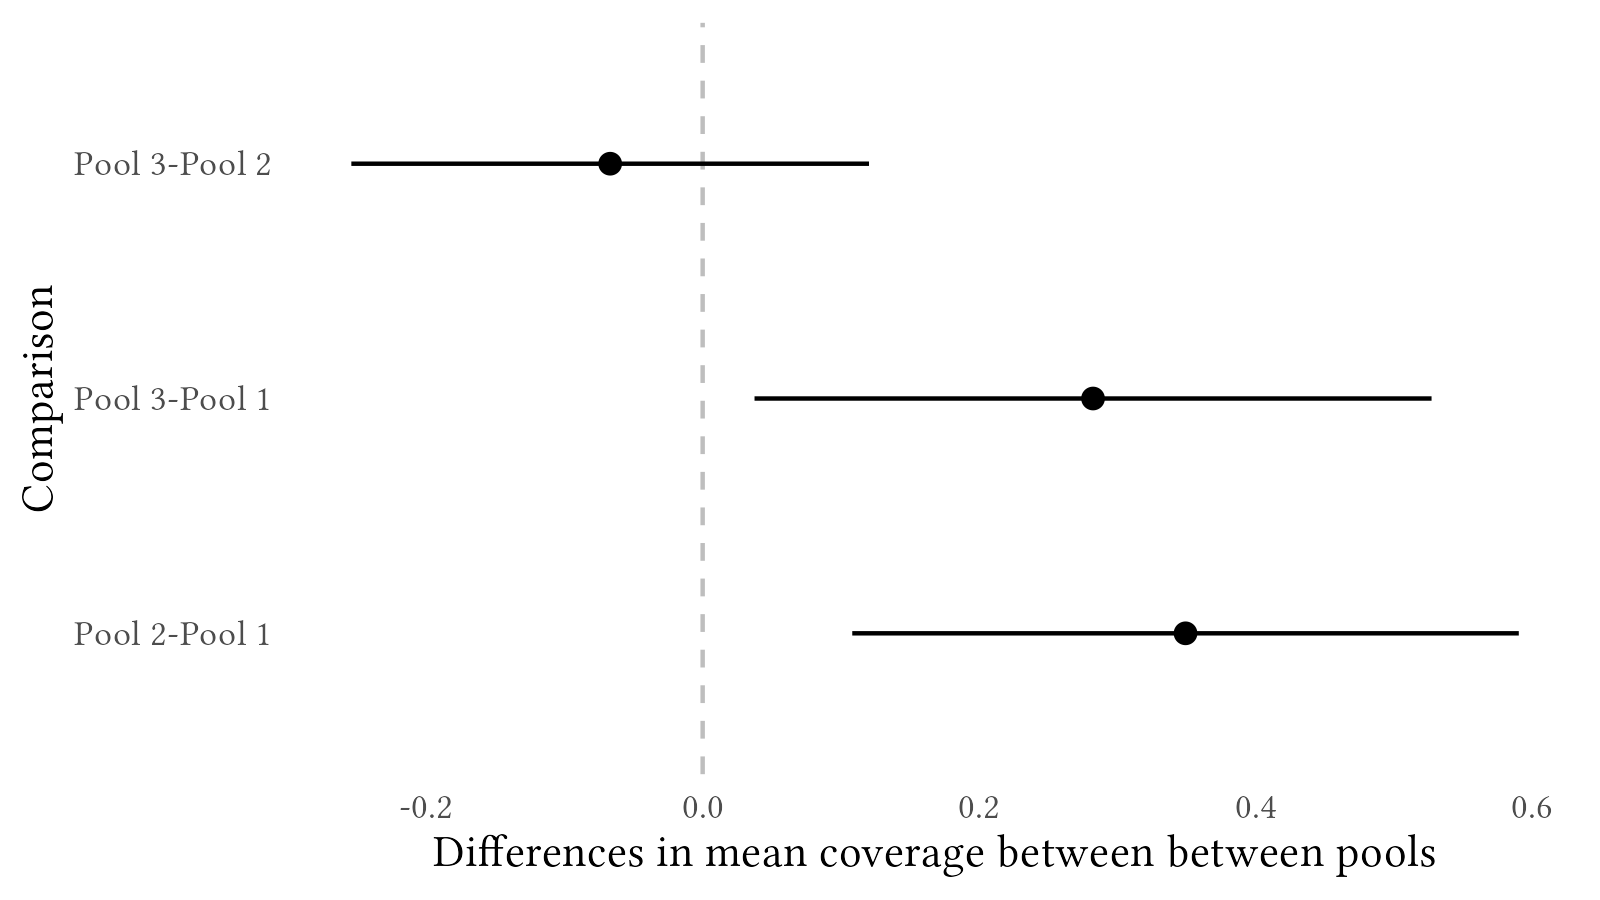
\includegraphics[width=\textwidth]{hsd_coverage_plot}
	\caption[Tukey \textsc{hsd} 95\% confidence intervals for tree cover]{Tukey \textsc{hsd} 95\% confidence intervals for tree cover.}
	\label{fig:hsd_coverage_plot}
\end{figure}

\clearpage
}



\clearpage


%}%Don't include if it doesn't exist.
%   ...
%% if Biographical sketch then
%    \begin{biosketch} ... \end{biosketch}
\end{document}